\documentclass[11pt,aspectratio=169]{beamer}

\usetheme{Madrid}
\usecolortheme{default}

\usepackage{amsmath,amsfonts,amssymb}
\usepackage{bm}
\usepackage{graphicx}
\usepackage{algorithm}
\usepackage{algpseudocode}
\usepackage{xspace}


% Theorem environments
\newtheorem{claim}[theorem]{Claim}
\newtheorem{prop}[theorem]{Proposition}
\newtheorem{empirical}[theorem]{Empirical Observation}

% Custom commands based on the paper
\newcommand{\lis}{{\tt lis}}
\newcommand{\loss}{{\tt loss}}
\newcommand{\est}{{\tt est}}
\newcommand{\bx}{Box}
\newcommand{\errorcont}{\Psi}
\newcommand{\RR}{\mathbb{R}}
\newcommand{\bmu}{\overline{\mu}}
% \newcommand{\bx}{Box}
\newcommand{\green}{Green}
\newcommand{\red}{Red}
\newcommand{\classifyb}{ClassifyBox}
\newcommand{\approxLIS}{\approxlis}
\newcommand{\sample}{Sample}

\newcommand{\len}{len}
\newcommand{\wt}{wt}
\newcommand{\st}{st}
\newcommand{\w}[1]{w(#1)}
\newcommand{\m}[1]{m(#1)}
\newcommand{\find}{Find}
\newcommand{\safe}{Safe}
\newcommand{\unsplit}{Unsplittable}
\newcommand{\tree}{tree}
\newcommand{\imp}{Improved}
\newcommand{\sparse}{Sparse}
% \newcommand{\lis}{{\tt lis}}
% \newcommand{\est}{{\tt est}}
% \newcommand{\loss}{{\tt loss}}
\newcommand{\alis}{{\tt alis}}
\newcommand{\aloss}{{\tt aloss}}
\newcommand{\lisloss}{\lambda}
\newcommand{\lossin}{{\tt loss_in}}
\newcommand{\inside}{{\tt in}}
\newcommand{\outside}{{\tt out}}
\newcommand{\phase}{{\tt ph}}
\newcommand{\In}{In}
\newcommand{\Out}{Out}
\newcommand{\leftedge}{{\bf{\rm LeftEdge}}}
\newcommand{\approxloss}{{\rm{\bf ApproxLoss}}}
\newcommand{\terminalbox}{{\rm{\bf TerminalBox}}}
\newcommand{\grid}{Grid}
\newcommand{\good}{Good}
\newcommand{\bad}{Bad}
\newcommand{\Bad}{Bad}
\newcommand{\Good}{Good}
\newcommand{\size}{Size}
\newcommand{\dead}{{\tt disposable}}
\newcommand{\spar}{{\tt sparse}}

\newcommand{\deltapar}{\overline{\delta}}
\newcommand{\deltaval}{1/\errorcont}
\newcommand{\err}{\xi}
\newcommand{\gridprecval}{\frac{1}{(C_2\errorcont)^4}}
\newcommand{\kappaest}{\widehat{\kappa}}
\newcommand{\suff}{{21}}
\newcommand{\sszval}{100\errorcont^3}
\newcommand{\taint}{\eta}
\newcommand{\taintval}{1/10\errorcont}
\newcommand{\taintprob}{\phi}
\newcommand{\taupar}{\overline{\tau}}


\newcommand{\lin}[2]{Line(#1^{(#2)})}
\newcommand{\move}[3]{#1^{(#2:#3)}}
\newcommand{\leftpar}{leftpar}
\newcommand{\nonleftpar}{nonleftpar}
\newcommand{\nlpath}{path}
\newcommand{\bdim}{dim}
\newcommand{\cyl}{cyl}
\newcommand{\pr}{{\rm Pr}}
\newcommand{\Sift}{{\em Sift}}
\newcommand{\Rep}{Rep}
\newcommand{\Linesift}{{\em Linesift}}
\newcommand{\Build}{{\em Build}}
\newcommand{\poly}{\textrm{poly}}
\newcommand{\p}{\mathcal{P}}
\newcommand{\mymod}{\textrm{mod} \ }
\newcommand{\otilde}{\widetilde{O}}
%\newcommand{\qed}{\hfill $\Box$}
\newcommand{\eps}{\varepsilon}
\newcommand{\fu}{\varphi}
\newcommand{\restr}[1]{{|_{{\textstyle #1}}}}
\newcommand{\proj}{\mbox{\rm proj}}
\newcommand{\vol}{\mbox{\tt vol}\,}
\newcommand{\area}{\mbox{\tt area}\,}
\newcommand{\conv}{\mbox{\tt conv}\,}
\newcommand{\diam}{\hbox{\tt diam}\,}
\newcommand{\hdisc}{\mbox{\rm herdisc}}
\newcommand{\ldisc}{\mbox{\rm lindisc}}
\newcommand{\EX}{\hbox{\bf E}}
\newcommand{\prob}{{\rm Prob}}
\newcommand{\proofend}{{\medskip\medskip}}
%\newcommand{\proof}{{\noindent\bf Proof: }}
\newcommand{\reals}{{\rm I\!\hspace{-0.025em} R}}
\newcommand{\dist}{\hbox{dist}}
\newcommand{\defeq}{\mbox{\,$\stackrel{\rm def}{=}$\,}}
\newcommand{\boxalg}[1]
{\begin{center}\fbox{\parbox{\columnwidth}{\tt
\begin{tabbing}
\=mm\=mm\=mm\=mm\=mm\=mm\=mm\=mm\=mm\kill
#1
\end{tabbing} } } \end{center} }
%%%%Mike's commands August 2010
\newcommand{\mass}{{\bf {\rm mass}}}
\newcommand{\viol}{{\bf {\rm  viol}}}
\newcommand{\strip}[2]{#1|#2}
\newcommand{\width}{{\bf {\rm  w}}}
\newcommand{\longpath}{{\bf {\rm Long-Path}}}
\newcommand{\errorprob}{\eps}
\newcommand{\spliterror}{\sigma}
\newcommand{\griderror}{\xi}
\newcommand{\gridprec}{\alpha}
\newcommand{\thresh}{\theta}
% \newcommand{\errorcont}{\Psi}
\newcommand{\numclaims}{6}
\newcommand{\neterror}{\xi}
\newcommand{\netprec}{\alpha}
\newcommand{\adderror}{\alpha}
%%%lossA  is the error introduced by step A in the analysis
\newcommand{\lossone}{\lambda_1}  
\newcommand{\losstwo}{\lambda_2}
\newcommand{\lossthree}{\lambda_3}
\newcommand{\lossfour}{\lambda_4}
\newcommand{\lossfive}{\lambda_5}
\newcommand{\losssix}{\lambda_6}
\newcommand{\lossseven}{\lambda_7}
\newcommand{\approxzero}{A_0}
\newcommand{\approxone}{A_1}
\newcommand{\approxtwo}{A_2}
\newcommand{\approxthree}{A_3}
\newcommand{\approxfour}{A_4}
\newcommand{\approxfive}{A_5}
\newcommand{\approxsix}{A_6}
\newcommand{\approxseven}{A_7}
\newcommand{\errorterm}{\zeta}
\newcommand{\errorzero}{\varepsilon_0}
\newcommand{\errorone}{\varepsilon_1}
\newcommand{\errortwo}{\varepsilon_2}
\newcommand{\errorthree}{\varepsilon_3}
\newcommand{\errorfour}{\varepsilon_4}
\newcommand{\errorfive}{\varepsilon_5}
\newcommand{\errorsix}{\varepsilon_6}
\newcommand{\errorseven}{\varepsilon_7}
\newcommand{\errorA}{\varepsilon_A}
\newcommand{\algcomment}[1]{$\backslash * \backslash$ {#1}}

\newcommand{\ssize}{{\bf {\tt sample\_size}}}
\newcommand{\ssz}{\sigma}
\newcommand{\rvmean}{\lambda}
\newcommand{\samplemean}{{\bf {\rm sample-mean}}}
\newcommand{\Estimate}{{\bf {\rm Estimate}}}
\newcommand{\criticalbox}{{\bf {\rm Critical-Box}}}
\newcommand{\constructcall}{{\bf {\rm Construct-Call}}}
\newcommand{\irrelevant}{{\bf {\rm Irrelevant}}}
\newcommand{\rightedge}{{\bf {\rm rightedge}}}
\newcommand{\classify}{{\rm {\bf Classify}}}
\newcommand{\LIS}{{\rm {\bf LIS}}}
\newcommand{\basicmain}{{\rm {\bf BasicMain}}}
\newcommand{\improvedmain}{{\rm {\bf ImprovedMain}}}
\newcommand{\approxlis}{{\rm {\bf ApproxLIS}}}
\newcommand{\approxlisfin}{{\rm {\bf FinalApproxLIS}}}
\newcommand{\critbox}{{\rm {\bf CriticalBox}}}
\newcommand{\leafbox}{{\sc LeafBox}}
\newcommand{\nextbox}{{\sc NextBox}}
\newcommand{\splitbox}{{\bf{\rm SplitBox}}}
\newcommand{\childbox}{{\rm {\bf ChildBox}}}
\newcommand{\findsplitter}{{\rm {\bf FindSplitter}}}
\newcommand{\splitterfound}{splitter\_found}
\newcommand{\buildgrid}{{\rm {\bf BuildGrid}}}
\newcommand{\buildnet}{{\rm {\bf BuildNet}}}
\newcommand{\lischain}{{\rm {\bf LIS.Chain}}}
\newcommand{\gridpath}{{\rm {\bf GridPath}}}
\newcommand{\gridchain}{{\rm {\bf GridChain}}}
\newcommand{\point}[2]{\langle #1,#2 \rangle}
\newcommand{\expressionone}{E_1}
\newcommand{\expressiontwo}{E_2}
\newcommand{\expressionthree}{E_3}
\newcommand{\expressionfour}{E_4}
\newcommand{\expressionfive}{E_5}
\newcommand{\expressionsix}{E_6}
\newcommand{\expressionseven}{E_7}
\newcommand{\expressioneight}{E_8}
\newcommand{\maxval}{{\tt valbound}}
\newcommand{\liserror}{\nu}


\title[Estimating LIS in Polylog Time]{Estimating the Longest Increasing Sequence in Polylogarithmic Time}
\subtitle{A Deep Dive into Sublinear Additive Approximations}
\author{Based on the paper by M. Saks and C. Seshadhri}
\date{Seminar Presentation}

\begin{document}

\begin{frame}
    \titlepage
\end{frame}

\begin{frame}{Outline (2-3 Hour Tutorial)}
    \tableofcontents[hideallsubsections]
\end{frame}

% =========================================================================
\section{Introduction and Background}
% =========================================================================

\begin{frame}{The Longest Increasing Subsequence (LIS) Problem}
    \begin{itemize}
        \item \textbf{Input:} A function $f:[n] \rightarrow \mathbb{R}$, which we view as an array.
        \item \textbf{Increasing Subsequence:} A sequence of indices $i_1 < i_2 < \cdots < i_k$ such that $f(i_1) \leq f(i_2) \leq \cdots \leq f(i_k)$.
        \item \textbf{Goal:} Find the length of the \emph{Longest Increasing Subsequence} (LIS).
        \pause
        \item \textbf{Classical Exact Algorithms:}
        \begin{itemize}
            \item Standard Dynamic Programming: $O(n^2)$.
            \item Fredman's Algorithm (1975): $O(n \log n)$ using an optimized DP.
            \item Patience Sorting (Aldous and Diaconis, 1999).
        \end{itemize}
    \end{itemize}
\end{frame}

\begin{frame}{Massive Datasets and Approximation}
    \begin{itemize}
        \item In the era of massive datasets, $O(n \log n)$ can be too slow if $n$ is enormous (e.g., streaming data, massive databases).
        \item \textbf{Question:} Can we estimate the LIS length in \emph{sublinear} or even \emph{polylogarithmic} time?
        \pause
        \item In sublinear algorithms, we access the array via queries to indices.
        \item We seek an approximate answer by observing a tiny, randomly chosen fraction of the array.
    \end{itemize}
\end{frame}

\begin{frame}{Distance to Monotonicity}
    \begin{itemize}
        \item We denote the LIS length as $\lis_f$.
        \item The \emph{complement} of the LIS is the \textbf{distance to monotonicity}: $\loss_f = n - \lis_f$.
        \item This represents the minimum number of values to change to make $f$ monotonically non-decreasing.
        \item \textbf{Normalized distance:} $\epsilon_f = \loss_f / n$.
    \end{itemize}
\end{frame}

\begin{frame}{Previous Work in Property Testing}
    \begin{itemize}
        \item Property testing distinguishes between $\loss_f = 0$ (perfectly sorted) and $\loss_f \geq \epsilon n$.
        \item Requires $O(\epsilon^{-1} \log n)$ random samples (Ergun et al. 2000, Fischer 2004).
        \item \textbf{Estimating Distance:}
        \begin{itemize}
            \item Parnas, Ron, and Rubinfeld (2004) \& Ailon, Chazelle, Comandur, and Liu (2004) provided algorithms to estimate $\loss_f$.
            \item Both yielded a \textbf{multiplicative $(2+o(1))$-approximation} to $\loss_f$.
            \item Running time: $(\loss_f (\log n)/n)^{O(1)}$.
        \end{itemize}
    \end{itemize}
\end{frame}

\begin{frame}{The Gap in Previous Knowledge}
    \begin{itemize}
        \item What if $\lis_f$ is between $0$ and $n/2$?
        \item In this case, $\loss_f \geq n/2$. 
        \item A factor-2 approximation to $\loss_f$ might return an estimate of $n$.
        \item The trivial estimate $\loss_f \approx n$ implies $\lis_f \approx 0$.
        \item \textbf{Consequence:} Previous algorithms gave an additive $n/2$ approximation for $\lis_f$. They could not distinguish an array with LIS of size $n/4$ from an array with LIS of size $o(n)$.
    \end{itemize}
\end{frame}

\begin{frame}{Main Result: Additive Approximation (Theorem 1.1)}
    \begin{block}{Theorem 1.1}
        There is a randomized algorithm which takes as input an array $f$ of size $n$ and parameter $\delta > 0$, and outputs a number $\est$ such that:
        $$|\est - \lis_f| \leq \delta n$$
        with probability at least $3/4$.
    \end{block}
    \begin{itemize}
        \item \textbf{Running Time:} $(1/\delta)^{O(1/\delta)} (\log n)^c$, for some absolute constant $c$.
        \item For any constant $\delta$, this is strictly \emph{polylogarithmic} in $n$.
    \end{itemize}
\end{frame}

\begin{frame}{Main Result: Distance to Monotonicity (Theorem 1.2)}
    \begin{block}{Theorem 1.2}
        Let $0 < \tau < 1$. There exists an algorithm with running time $(1/(\epsilon_f\tau))^{O(1/\tau)}(\log n)^c$ that computes $\epsilon$ such that:
        $$\epsilon_f \in [\epsilon, (1+\tau)\epsilon]$$
        with probability at least $3/4$.
    \end{block}
    \begin{itemize}
        \item Improves the previous $(2+o(1))$-approximation to a $(1+\tau)$-approximation!
    \end{itemize}
\end{frame}

% =========================================================================
\section{Obstacles to Additive Estimations}
% =========================================================================

\begin{frame}{Why is this hard? Obstacle 1: Uniform Sampling}
    \begin{itemize}
        \item \textbf{Na\"ive approach:} Take a random sample $S$, compute $\lis_f(S)$ exactly, scale up by $n/|S|$.
        \item \textbf{Failure Case:}
        \begin{center}
            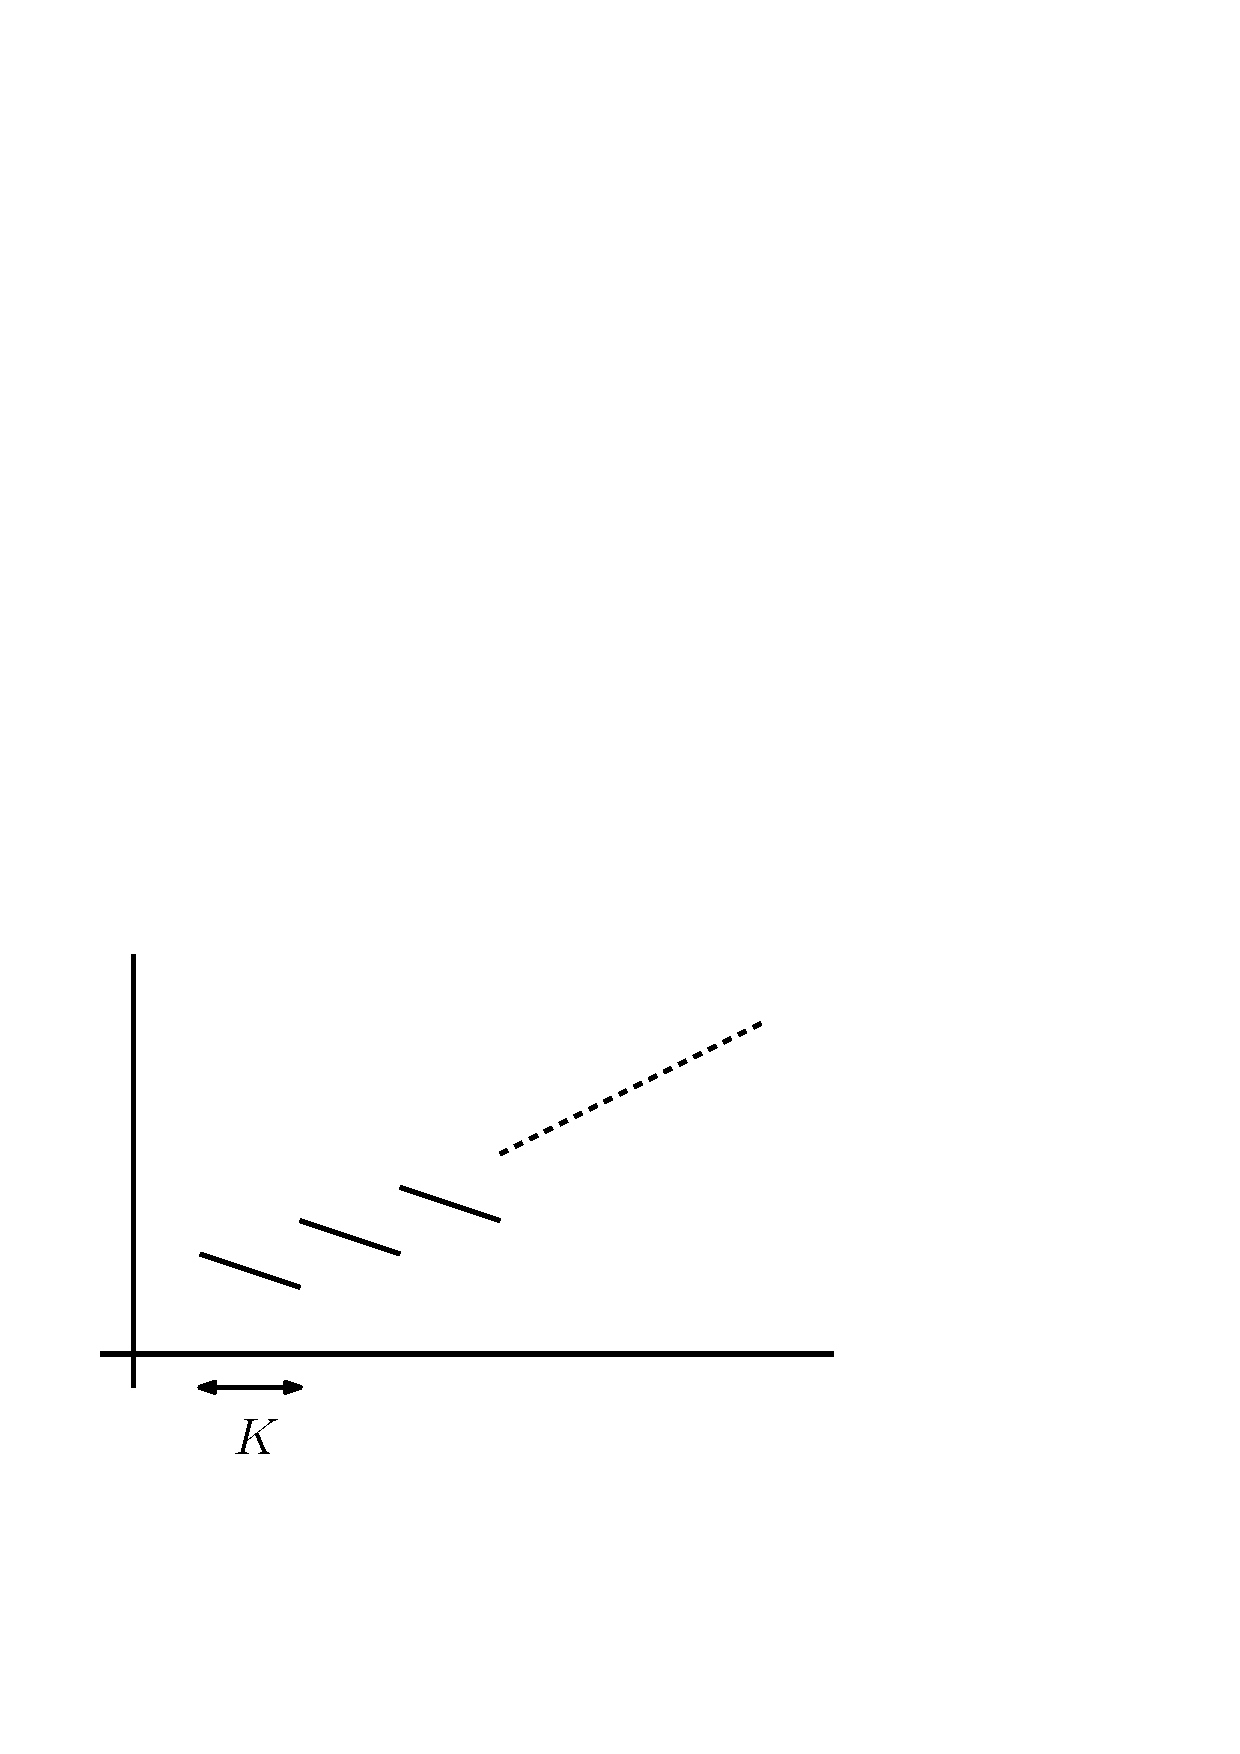
\includegraphics[width=0.2\textwidth]{figures/func1.pdf}
        \end{center}
        \item Array consists of blocks of size $K$. Within a block, items are decreasing. Blocks are globally increasing.
        \item $\lis_f = n/K$.
        \item A small uniform sample will almost certainly pick at most 1 item per block, looking \emph{completely increasing}. The estimate will be $\approx n$.
    \end{itemize}
\end{frame}

\begin{frame}{Obstacle 2: Proximity-Based Sampling}
    \begin{itemize}
        \item \textbf{Previous strategy (ACCL, PRR):} Classify each index as \emph{good} or \emph{bad}.
        \item For an index $i$, sample points $j$ with probability $\propto 1/|i-j|$. If $i$ has many violations with the sample, classify it as \emph{bad}.
        \item \textbf{Failure Case:}
        \begin{center}
            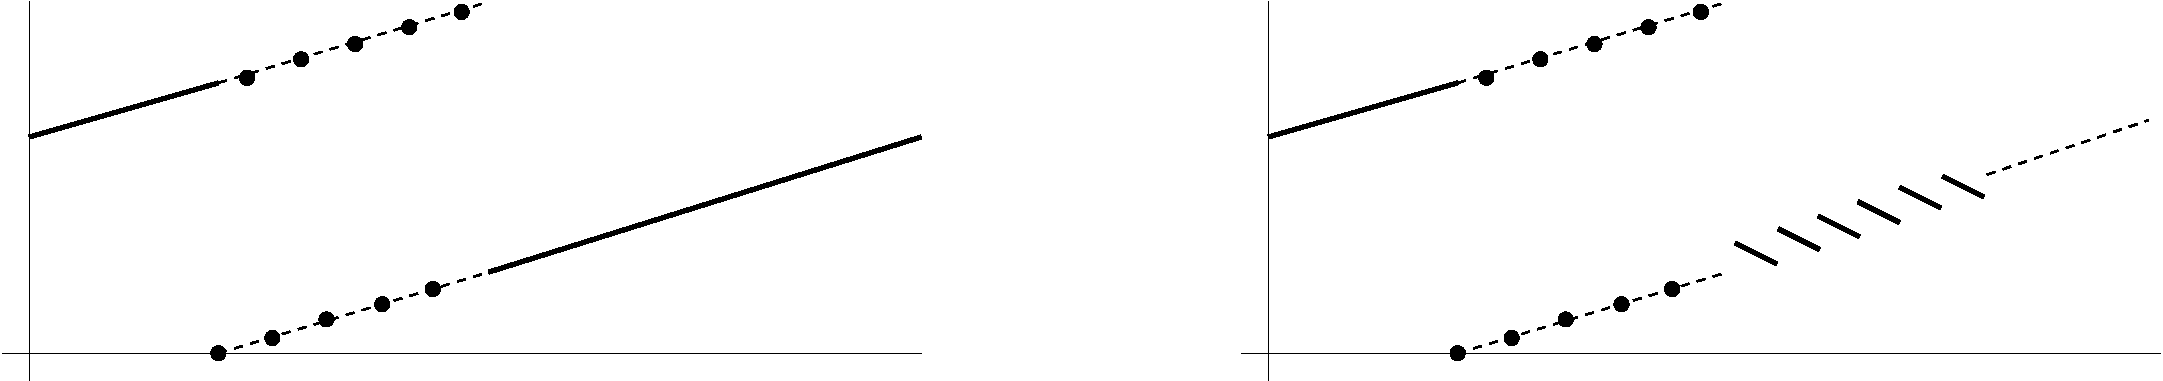
\includegraphics[width=0.2\textwidth]{figures/func-f.pdf}
        \end{center}
        \item A block's local classification may depend on small-scale properties \emph{far away} from it. Local/proximity sampling cannot see the correct global alignment.
        \item Conclusion: We need a mechanism that links global structure across all scales.
    \end{itemize}
\end{frame}

% =========================================================================
\section{Algorithmic Intuition}
% =========================================================================

\begin{frame}{An Interactive Protocol (Thought Experiment)}
    \begin{itemize}
        \item Imagine an all-knowing \textbf{Prover} and a bounded \textbf{Verifier}.
        \item Prover claims $\lis_f \geq bn$. 
        \item \textbf{Round:}
        \begin{enumerate}
            \item Verifier picks a random index $i \in [n]$. Let $F(i) = \langle i, f(i) \rangle$.
            \item They iteratively shrink a "bounding box". Prover offers a \emph{splitter} $S_j$.
            \item Verifier checks if $F(i)$ is comparable to $S_j$. If not, reject!
            \item Depending on $F(i) \preceq S_j$ or $F(i) \succ S_j$, they narrow the box to the bottom-left or top-right.
        \end{enumerate}
    \end{itemize}
\end{frame}

\begin{frame}{Interactive Protocol Visualized}
    \begin{center}
        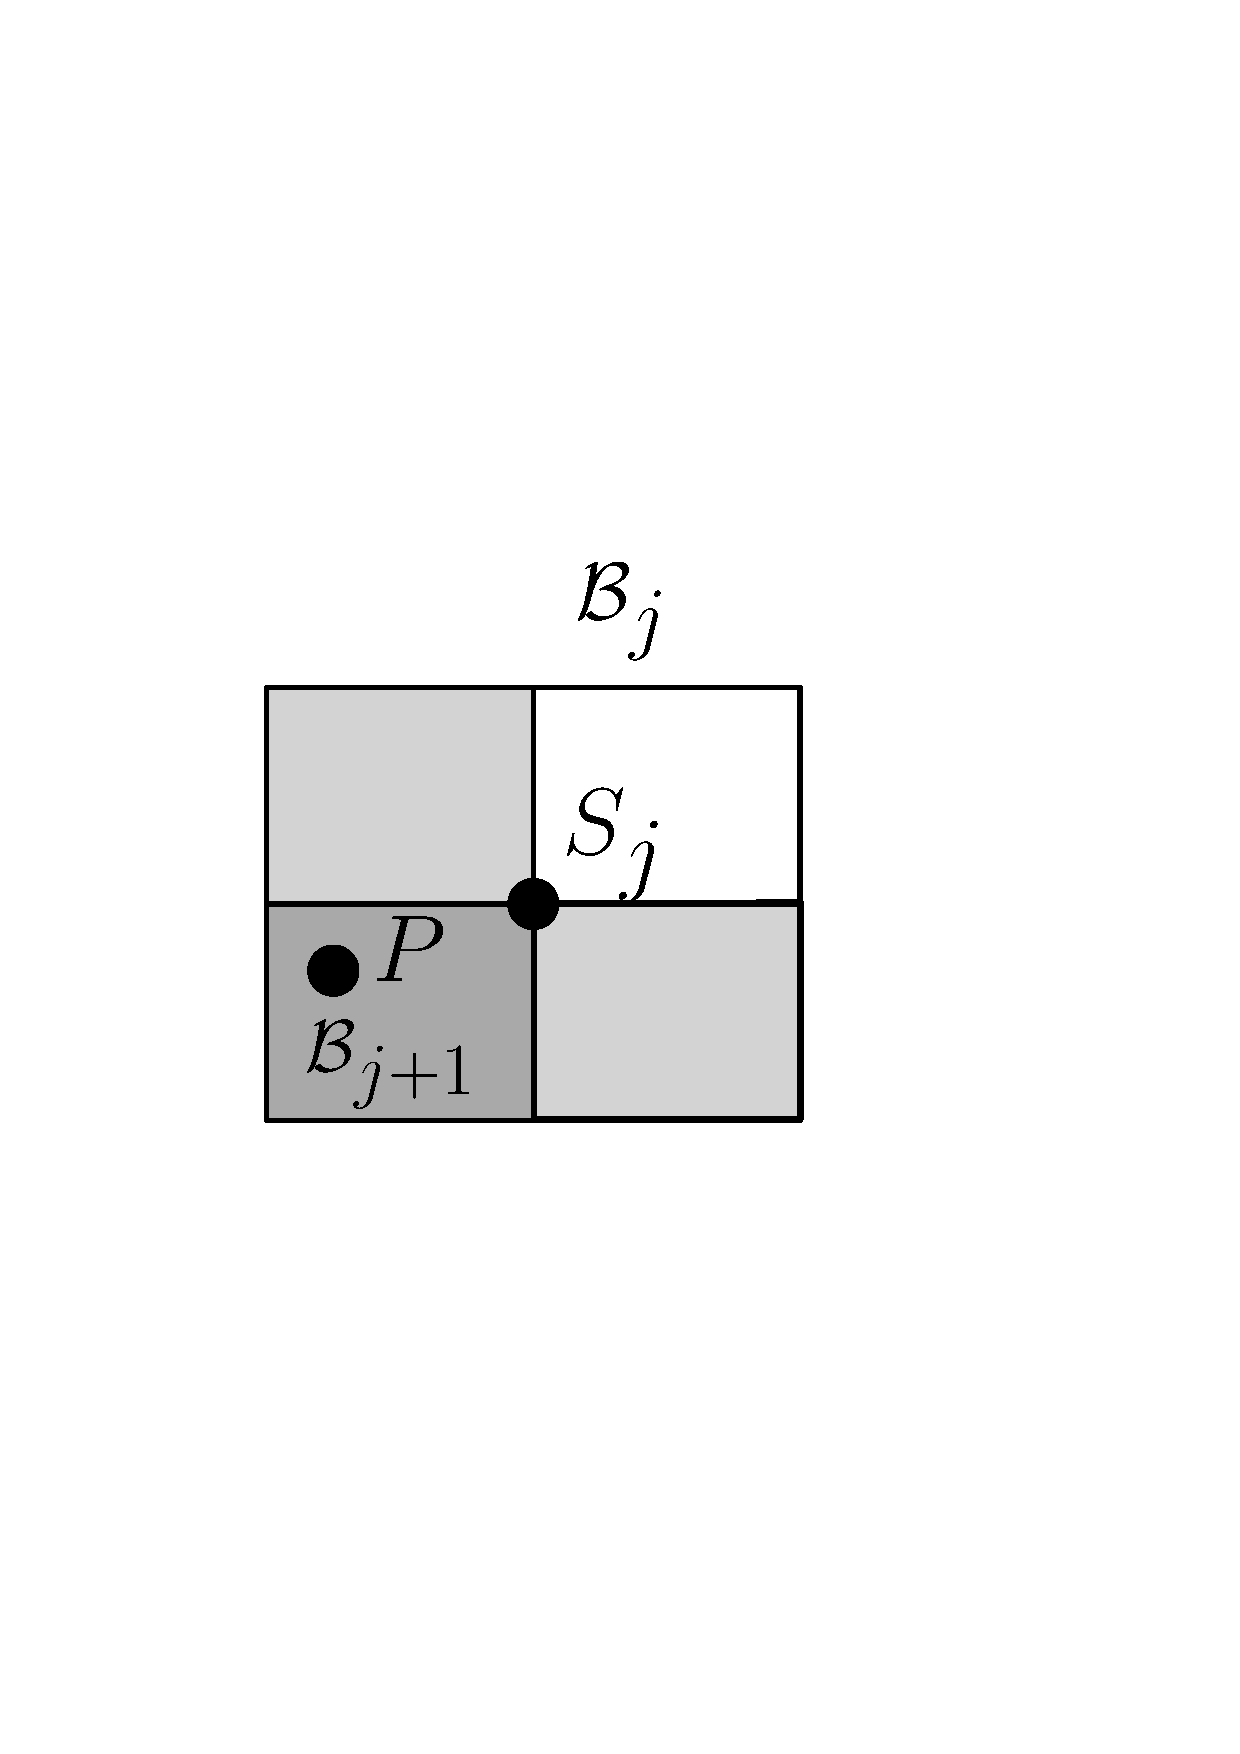
\includegraphics[width=0.3\textwidth]{figures/protocol.pdf}
    \end{center}
    \begin{itemize}
        \item If $F(i)$ is in the light gray regions, it's incomparable to $S_j$. Verifier rejects.
        \item If the Prover is honest (LIS is large), they can pick splitters directly from the true LIS, and the Verifier accepts with probability $\geq b$.
    \end{itemize}
\end{frame}

\begin{frame}{Simulating the Prover without an Oracle}
    \begin{itemize}
        \item We don't have a Prover. How do we find a good splitter algorithmically?
        \item A good splitter $S$ has few \emph{violations} (incomparable points) with the unknown LIS.
        \item Since we don't know the LIS, we look for a \textbf{conservative splitter}: one that has few violations with \emph{all} points in the current box.
        \item If conservative splitters exist, random sampling can easily find one!
    \end{itemize}
\end{frame}

\begin{frame}{The Dichotomy: Splitter vs. Boosting}
    \begin{itemize}
        \item What if there are \emph{no} conservative splitters?
        \item \textbf{The Boosting Idea:}
        \begin{itemize}
            \item If an index $s$ causes many violations, we can use it to split the box $\mathcal{B}$ into $\mathcal{B}_L$ and $\mathcal{B}_R$.
            \item Recursively approximate $\lis(\mathcal{B}_L)$ and $\lis(\mathcal{B}_R)$.
            \item The number of points \emph{lost} (the violations) is precisely the difference between $\loss(\mathcal{B})$ and $\loss(\mathcal{B}_L) + \loss(\mathcal{B}_R)$.
            \item If there are many violations, we significantly \emph{boost} our approximation accuracy by dividing and conquering!
        \end{itemize}
        \item \textbf{Dichotomy:} Either a box has a good splitter (so we can efficiently narrow our search), or it has no good splitters (meaning dividing the box yields a strictly smaller accumulated error).
    \end{itemize}
\end{frame}

% =========================================================================
\section{Preliminaries and Definitions}
% =========================================================================

\begin{frame}{Points, Relations, and Boxes}
    \begin{itemize}
        \item \textbf{Points:} Represent indices and values as $P = \langle x, y \rangle \in \mathbb{N}^2$.
        \item $F(x) = \langle x, f(x) \rangle$. $\mathcal{F}$ is the set of all such points.
        \item \textbf{Relations:}
        \begin{itemize}
            \item $P \preceq Q$: $x(P) \leq x(Q)$ and $y(P) \leq y(Q)$.
            \item $P \prec Q$: $x(P) < x(Q)$ and $y(P) \leq y(Q)$.
            \item $P \searrow Q$: $x(P) < x(Q)$ and $y(P) > y(Q)$ (a \emph{violation}).
        \end{itemize}
        \item \textbf{Regions:} $P^{NW}, P^{SW}, P^{NE}, P^{SE}$.
        \begin{center}
            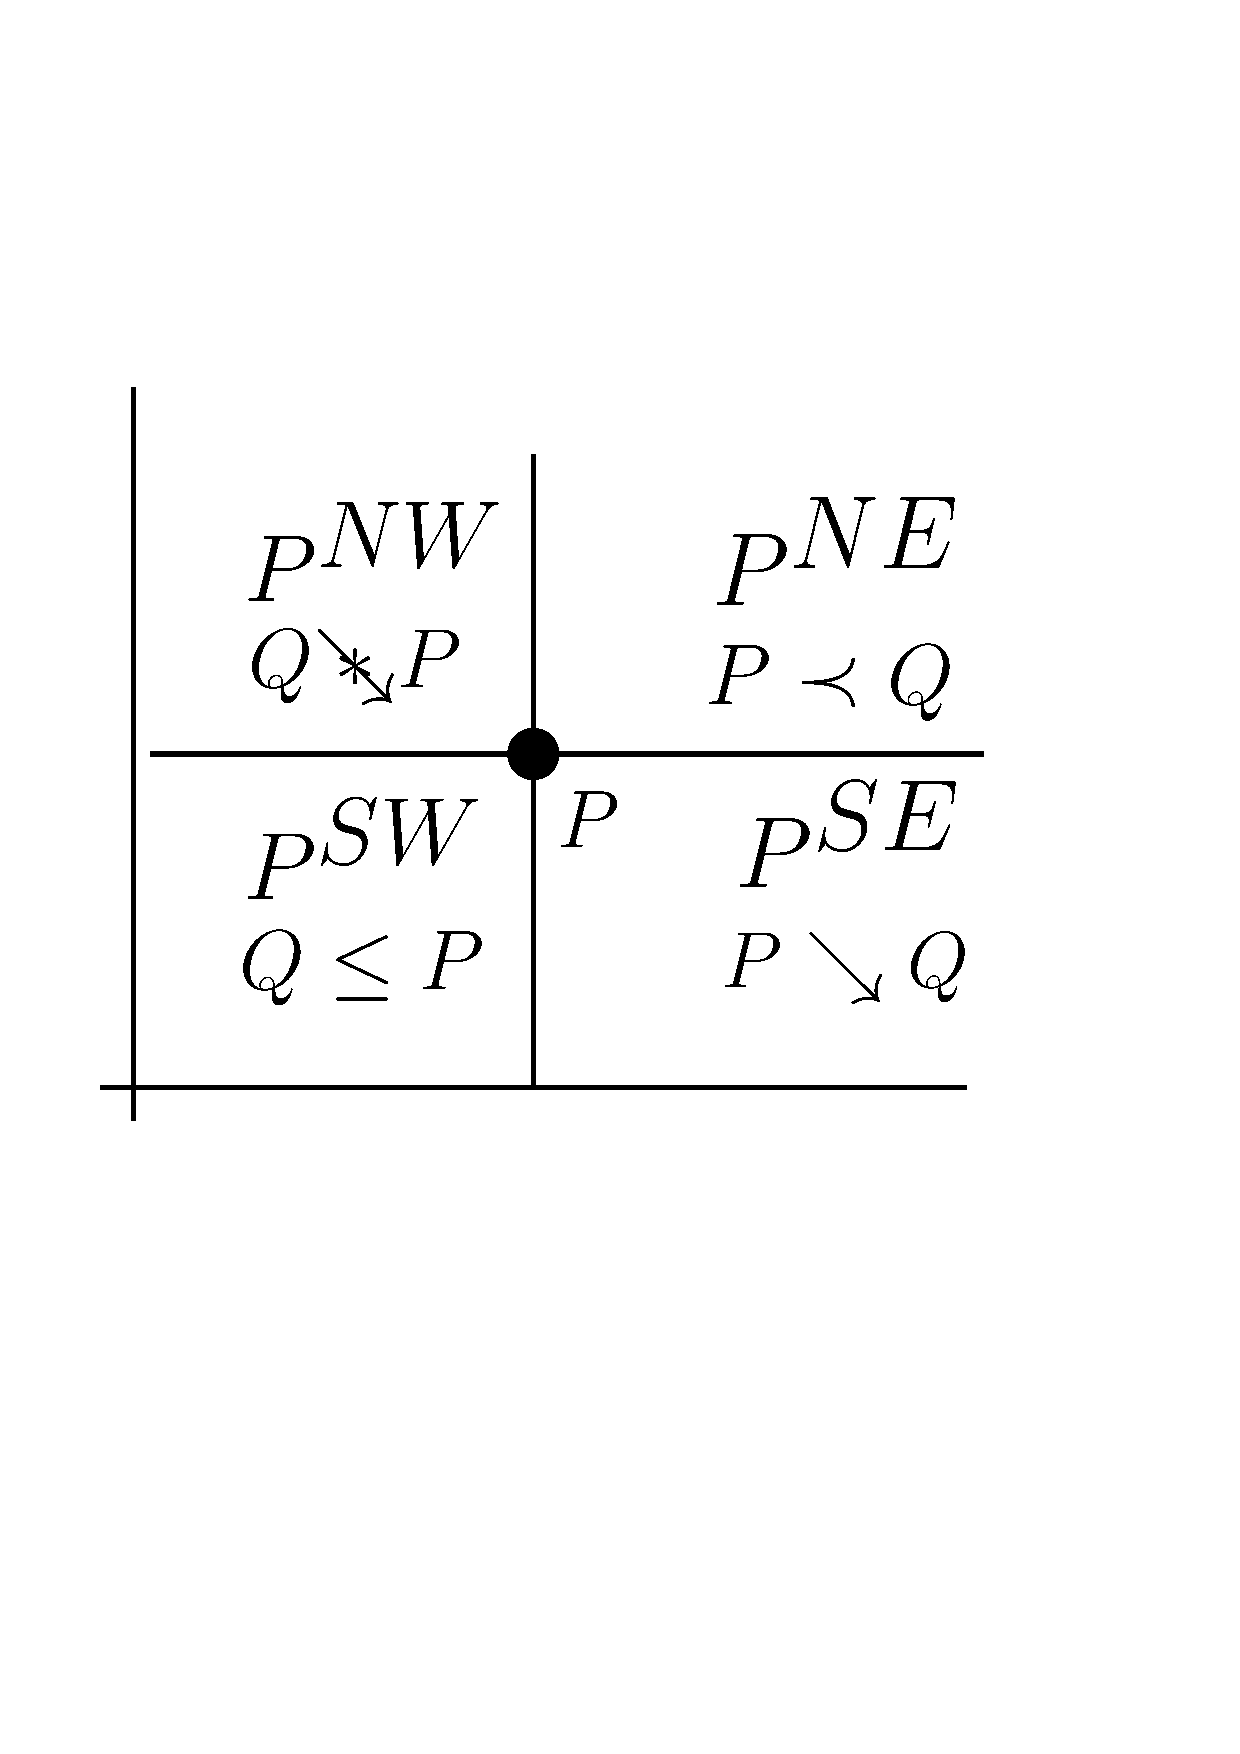
\includegraphics[width=0.3\textwidth]{figures/position.pdf}
        \end{center}
    \end{itemize}
\end{frame}

\begin{frame}{Boxes and Box Chains}
    \begin{itemize}
        \item \textbf{Box} $\mathcal{B}$: A Cartesian product of an index interval and value interval.
        \item \textbf{Box Sequence:} $\vec{\mathcal{B}} = (\mathcal{B}_1, \dots, \mathcal{B}_k)$ where each is strictly to the right of the previous.
        \item \textbf{Box Chain:} A sequence where the top-right of $\mathcal{B}_i$ is exactly the bottom-left of $\mathcal{B}_{i+1}$.
        \begin{center}
            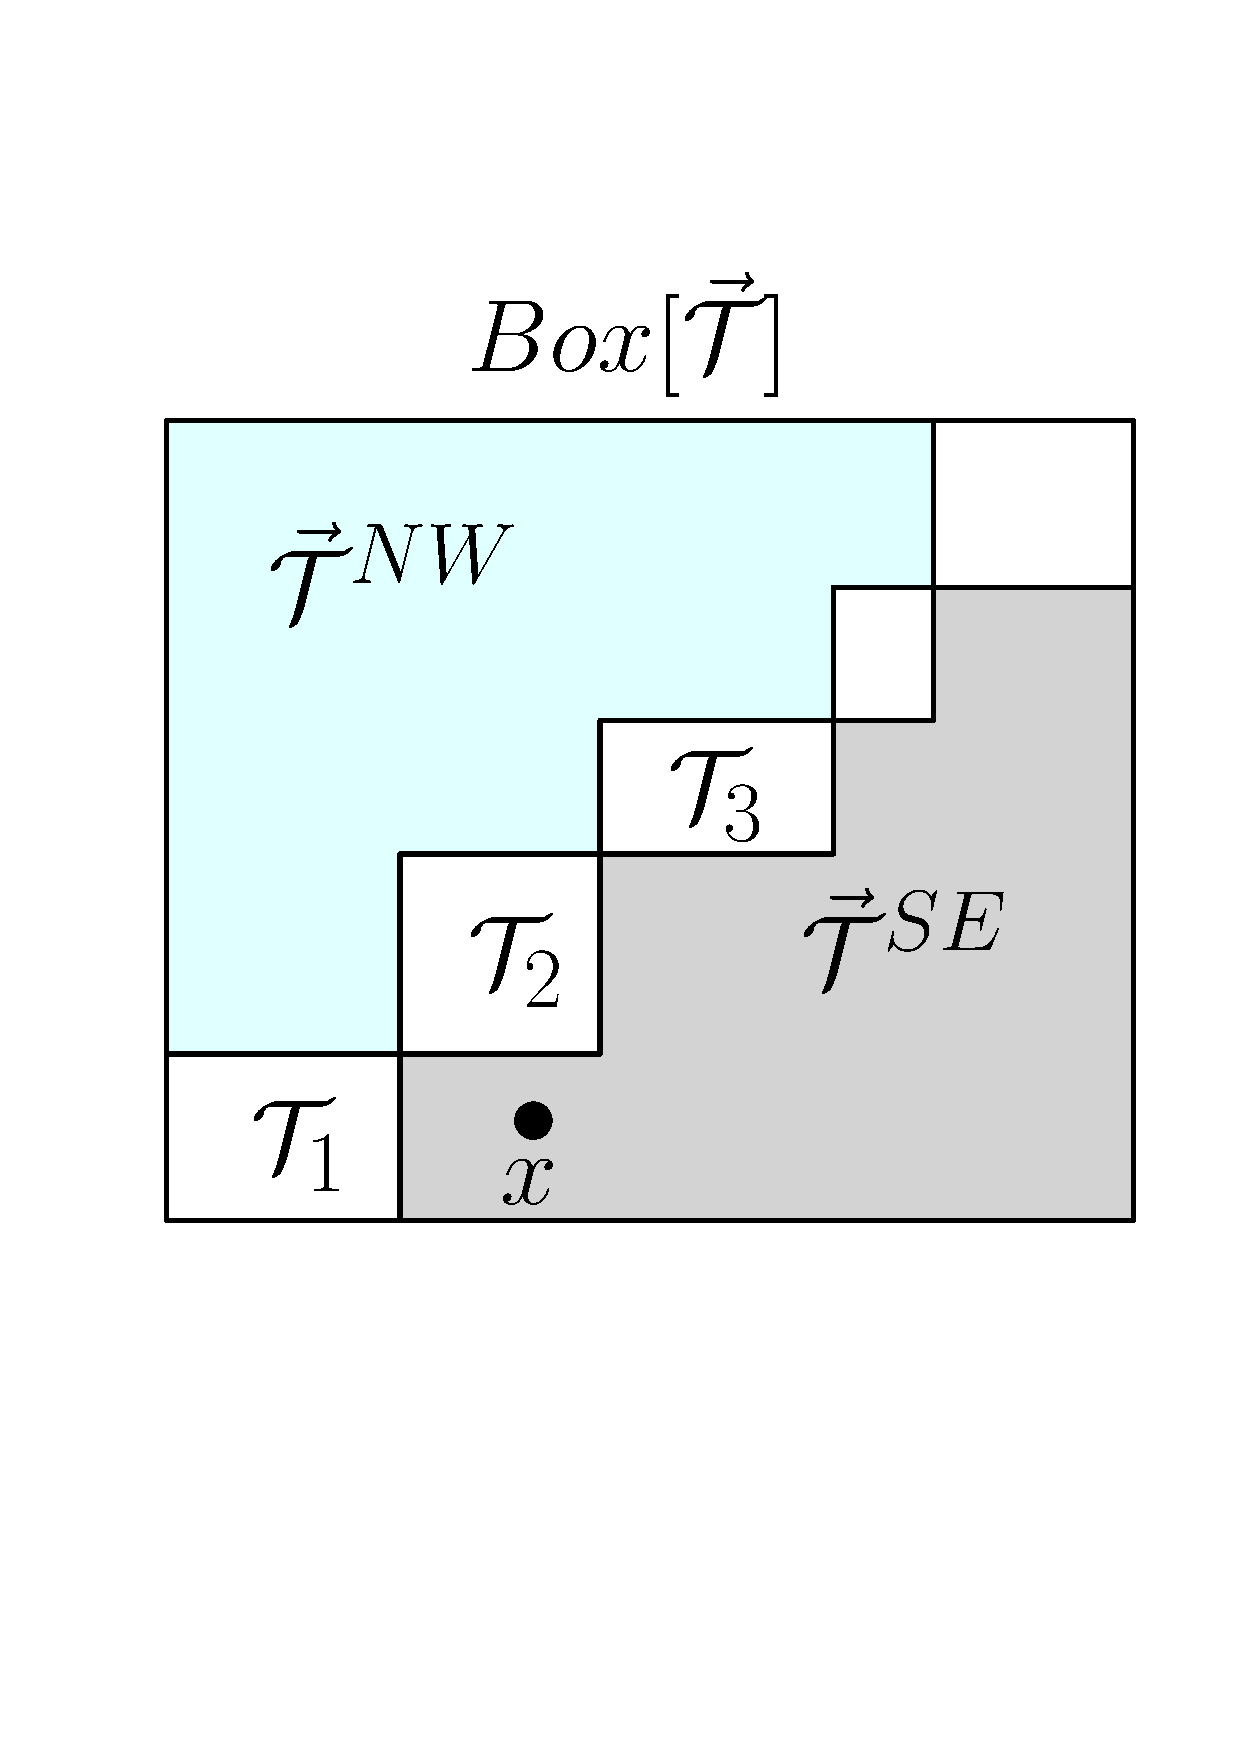
\includegraphics[width=0.2\textwidth]{figures/boxchain.pdf}
        \end{center}
        \item An increasing sequence of points defines a box chain, and vice versa.
    \end{itemize}
\end{frame}

\begin{frame}{Strips and The Functions \lis and \loss}
    \begin{itemize}
        \item \textbf{$\mathcal{B}$-strip:} A subbox $\mathcal{S}$ of $\mathcal{B}$ that has the same vertical extent as $\mathcal{B}$.
        \begin{center}
            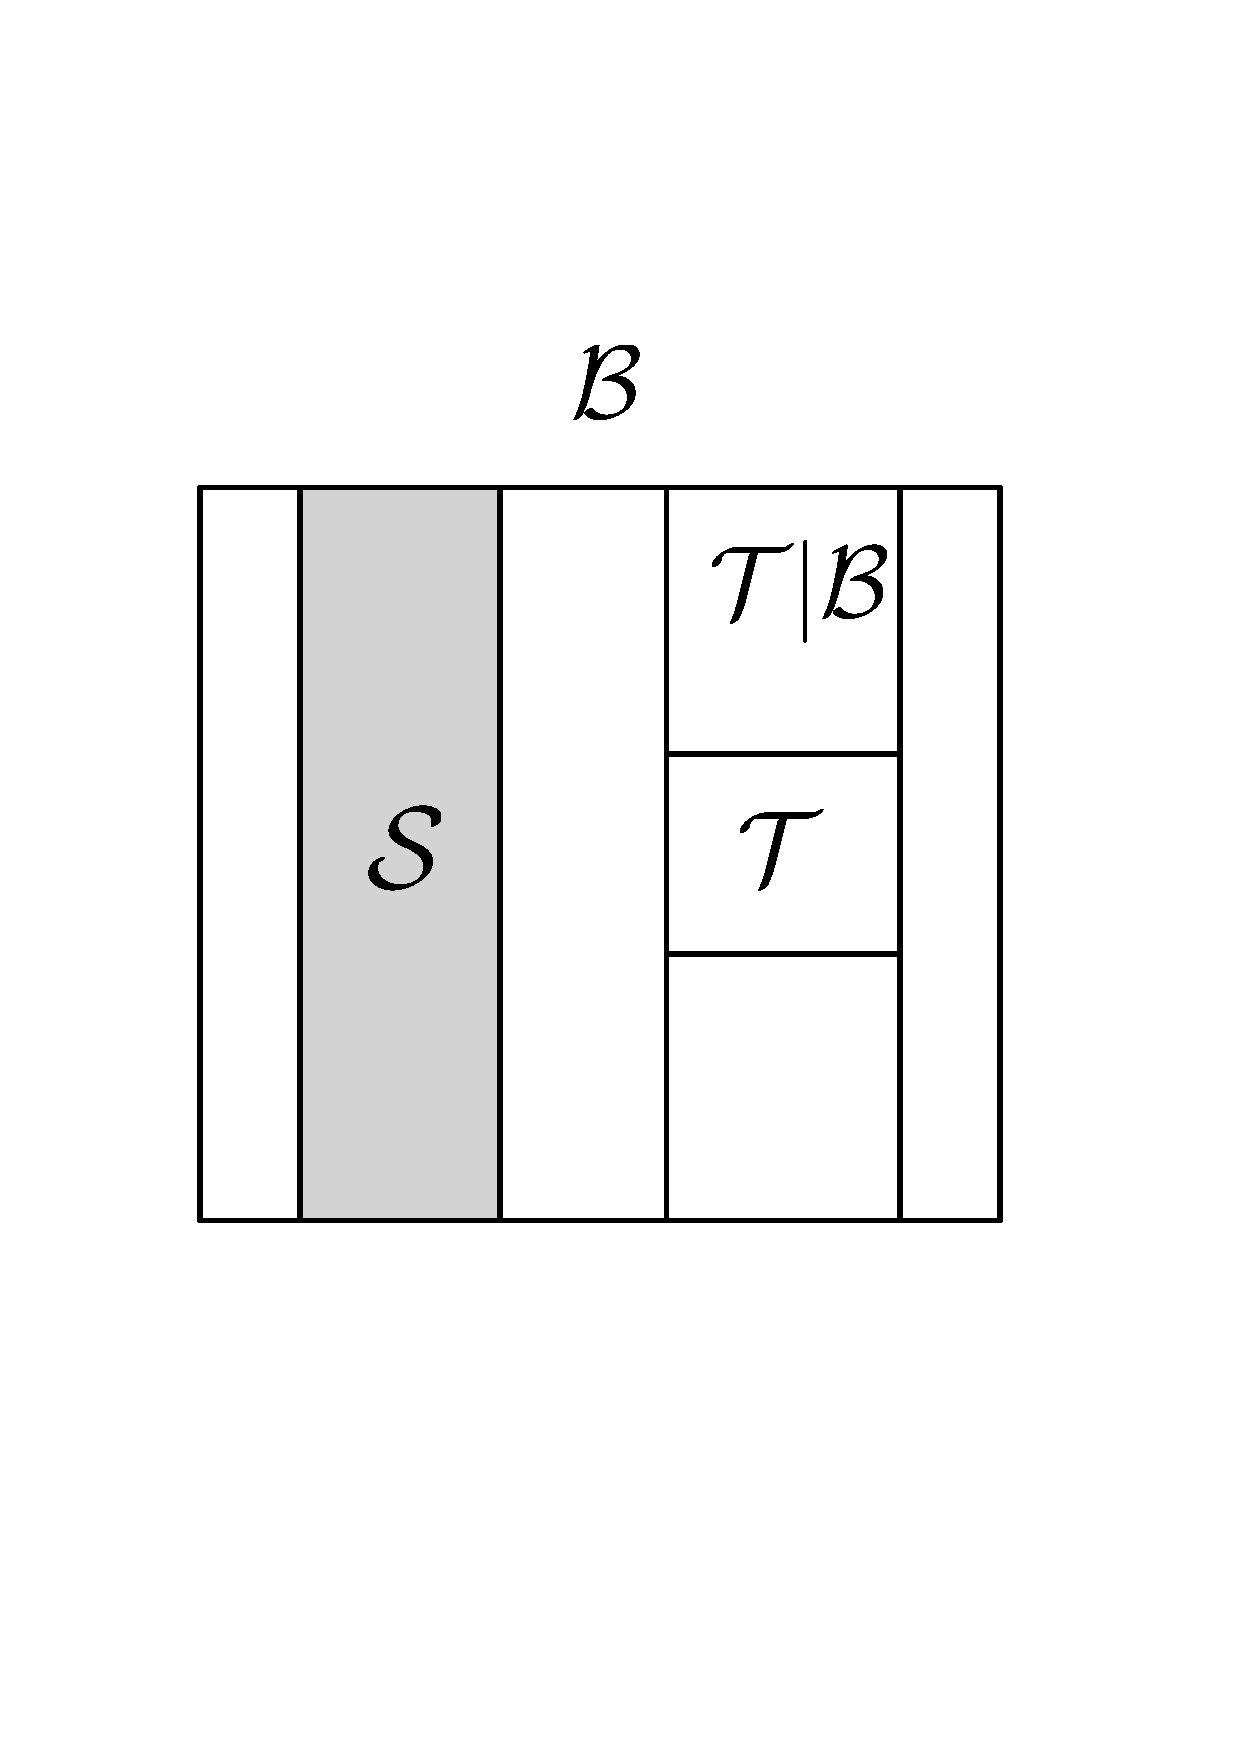
\includegraphics[width=0.2\textwidth]{figures/strip.pdf}
        \end{center}
        \item $\lis(\mathcal{B})$: Size of the longest increasing sequence of $\mathcal{F}$-points contained entirely in $\mathcal{B}$.
        \item $\loss(\mathcal{B}) = |\mathcal{B} \cap \mathcal{F}| - \lis(\mathcal{B})$.
    \end{itemize}
\end{frame}

\begin{frame}{The Approximation Goal}
    \begin{itemize}
        \item We want an algorithm $\approxlis(\mathcal{B})$ that returns an approximation.
        \item We measure error using two parameters: \textbf{Primary Error} ($\tau$) and \textbf{Secondary Error} ($\delta$).
        \item \textbf{Target:} 
        $$|\approxlis(\mathcal{B}) - \lis(\mathcal{B})| \leq \tau \cdot \loss(\mathcal{B}) + \delta \cdot \width(\mathcal{B})$$
        \item $\tau$ will decrease with recursive depth, while $\delta$ will increase. We manage these to bound total error.
    \end{itemize}
\end{frame}

% =========================================================================
\section{Algorithmic Building Blocks}
% =========================================================================

\begin{frame}{Building Block 1: Finding Splitters}
    \begin{itemize}
        \item A \textbf{splitter} $s$ divides a box $\mathcal{T}$ into a bottom-left box and a top-right box.
        \item We want a splitter that is:
        \begin{enumerate}
            \item \textbf{Balanced:} Not too close to the left or right edge (parameter $\rho$).
            \item \textbf{Safe:} The number of violations inside any adjacent strip $\mathcal{S}$ is at most $L + \mu |\mathcal{F} \cap \mathcal{S}|$.
        \end{enumerate}
        \item $\findsplitter(\mathcal{T}, \mathcal{B}, \mu, L, \rho)$:
        \begin{itemize}
            \item Randomly sample $O(\log^2 n / \rho)$ balanced points.
            \item Use secondary sampling to estimate violations.
            \item Return an adequate splitter if one is found.
        \end{itemize}
    \end{itemize}
\end{frame}

\begin{frame}{The Dichotomy Lemma (The Theoretical Heart)}
    \begin{itemize}
        \item What if $\findsplitter$ fails?
        \item Let $\mathcal{R}$ be a box, $\vec{\mathcal{S}}$ a strip decomposition, $\vec{\mathcal{D}}$ a box chain compatible with $\vec{\mathcal{S}}$.
        \item Let $U$ be the set of "unsafe" indices inside $\vec{\mathcal{D}}$.
        \item Let $\chi = |\mathcal{R} \cap \mathcal{F}|$, $\chi^{in}$ points inside $\vec{\mathcal{D}}$, $\chi^{out}$ points outside $\vec{\mathcal{D}}$.
    \end{itemize}
    \begin{block}{Lemma 4.6 (Dichotomy)}
        $$\chi^{out} \geq \frac{\mu}{1-\mu} |U|$$
        $$\chi^{in} \leq (1-\mu)\chi + \mu |S|$$
        where $S$ is the set of safe points.
    \end{block}
\end{frame}

\begin{frame}{Dichotomy Lemma Visualization}
    \begin{center}
        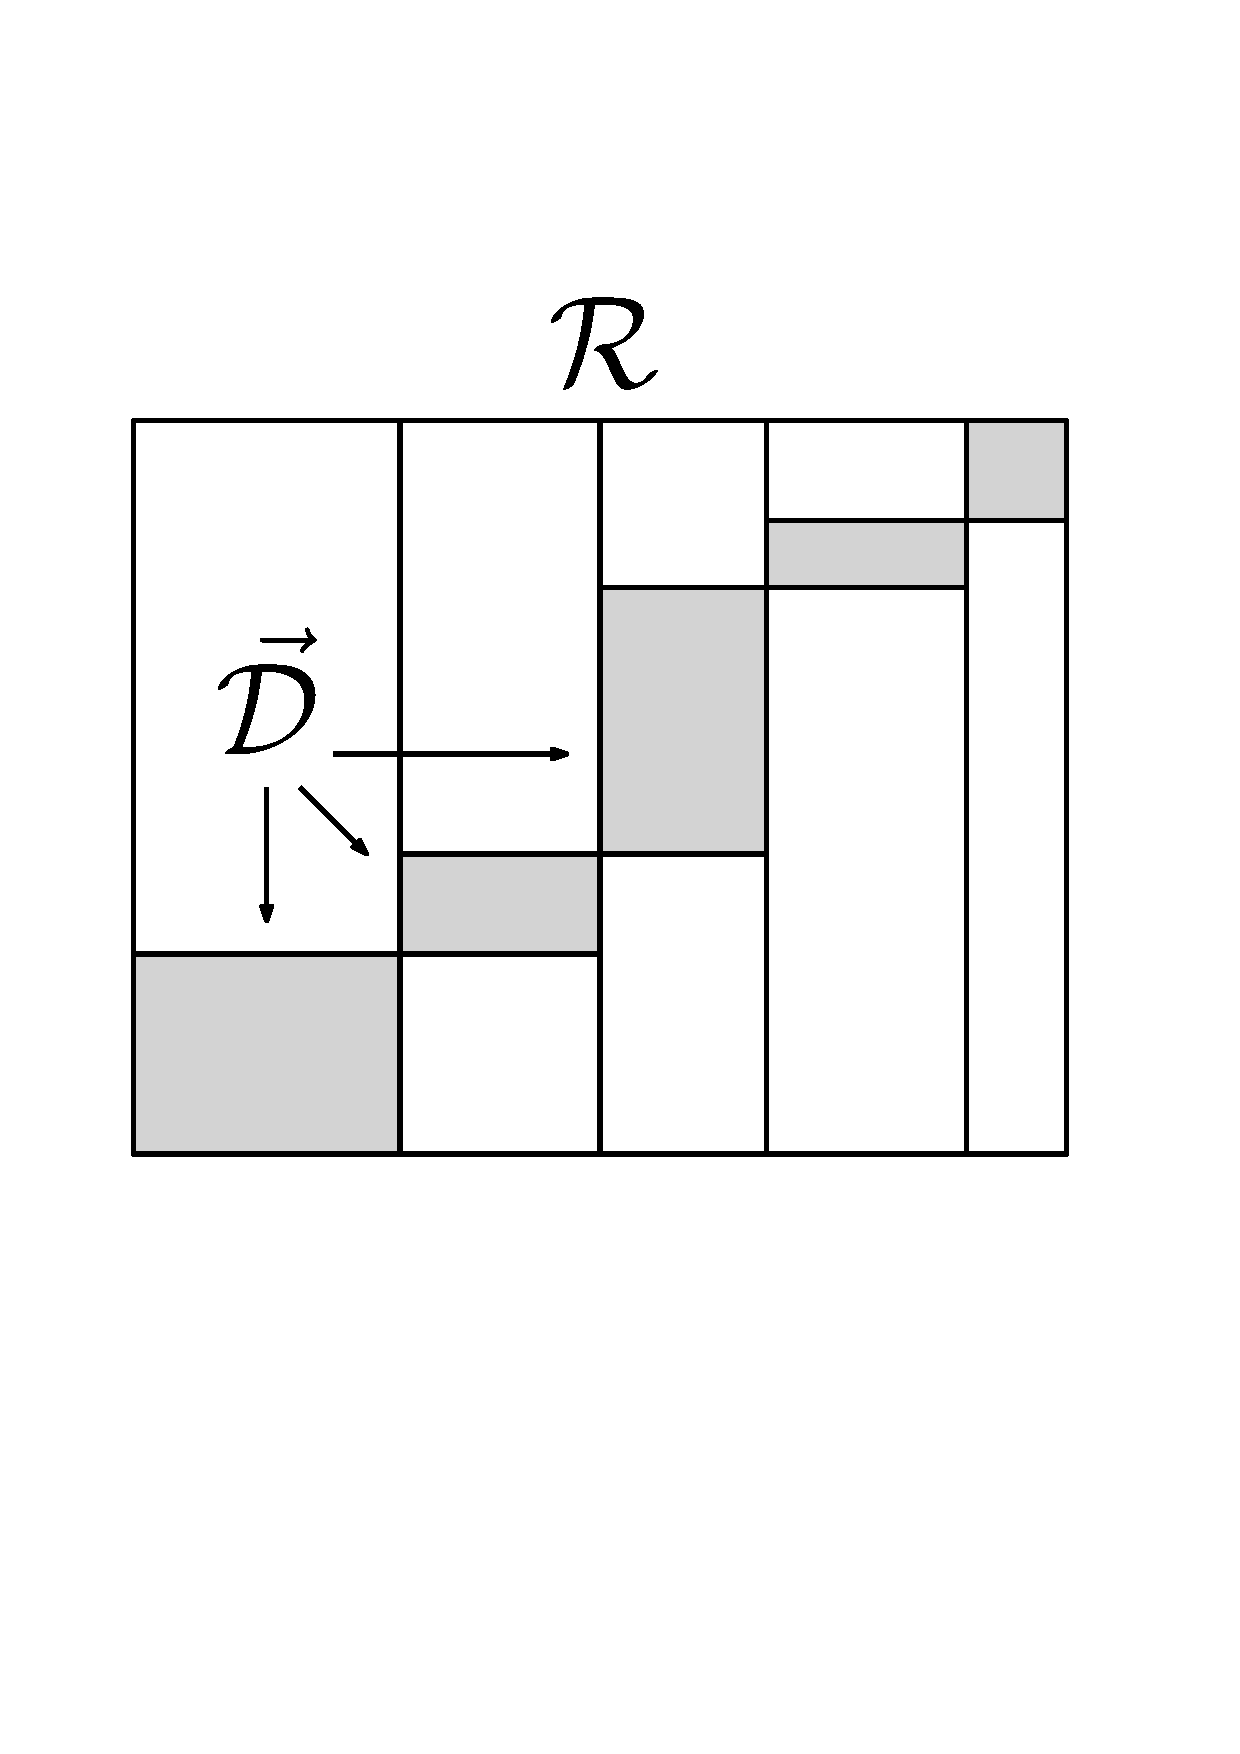
\includegraphics[width=0.2\textwidth]{figures/dichotomy1.pdf} \hspace{1cm}
        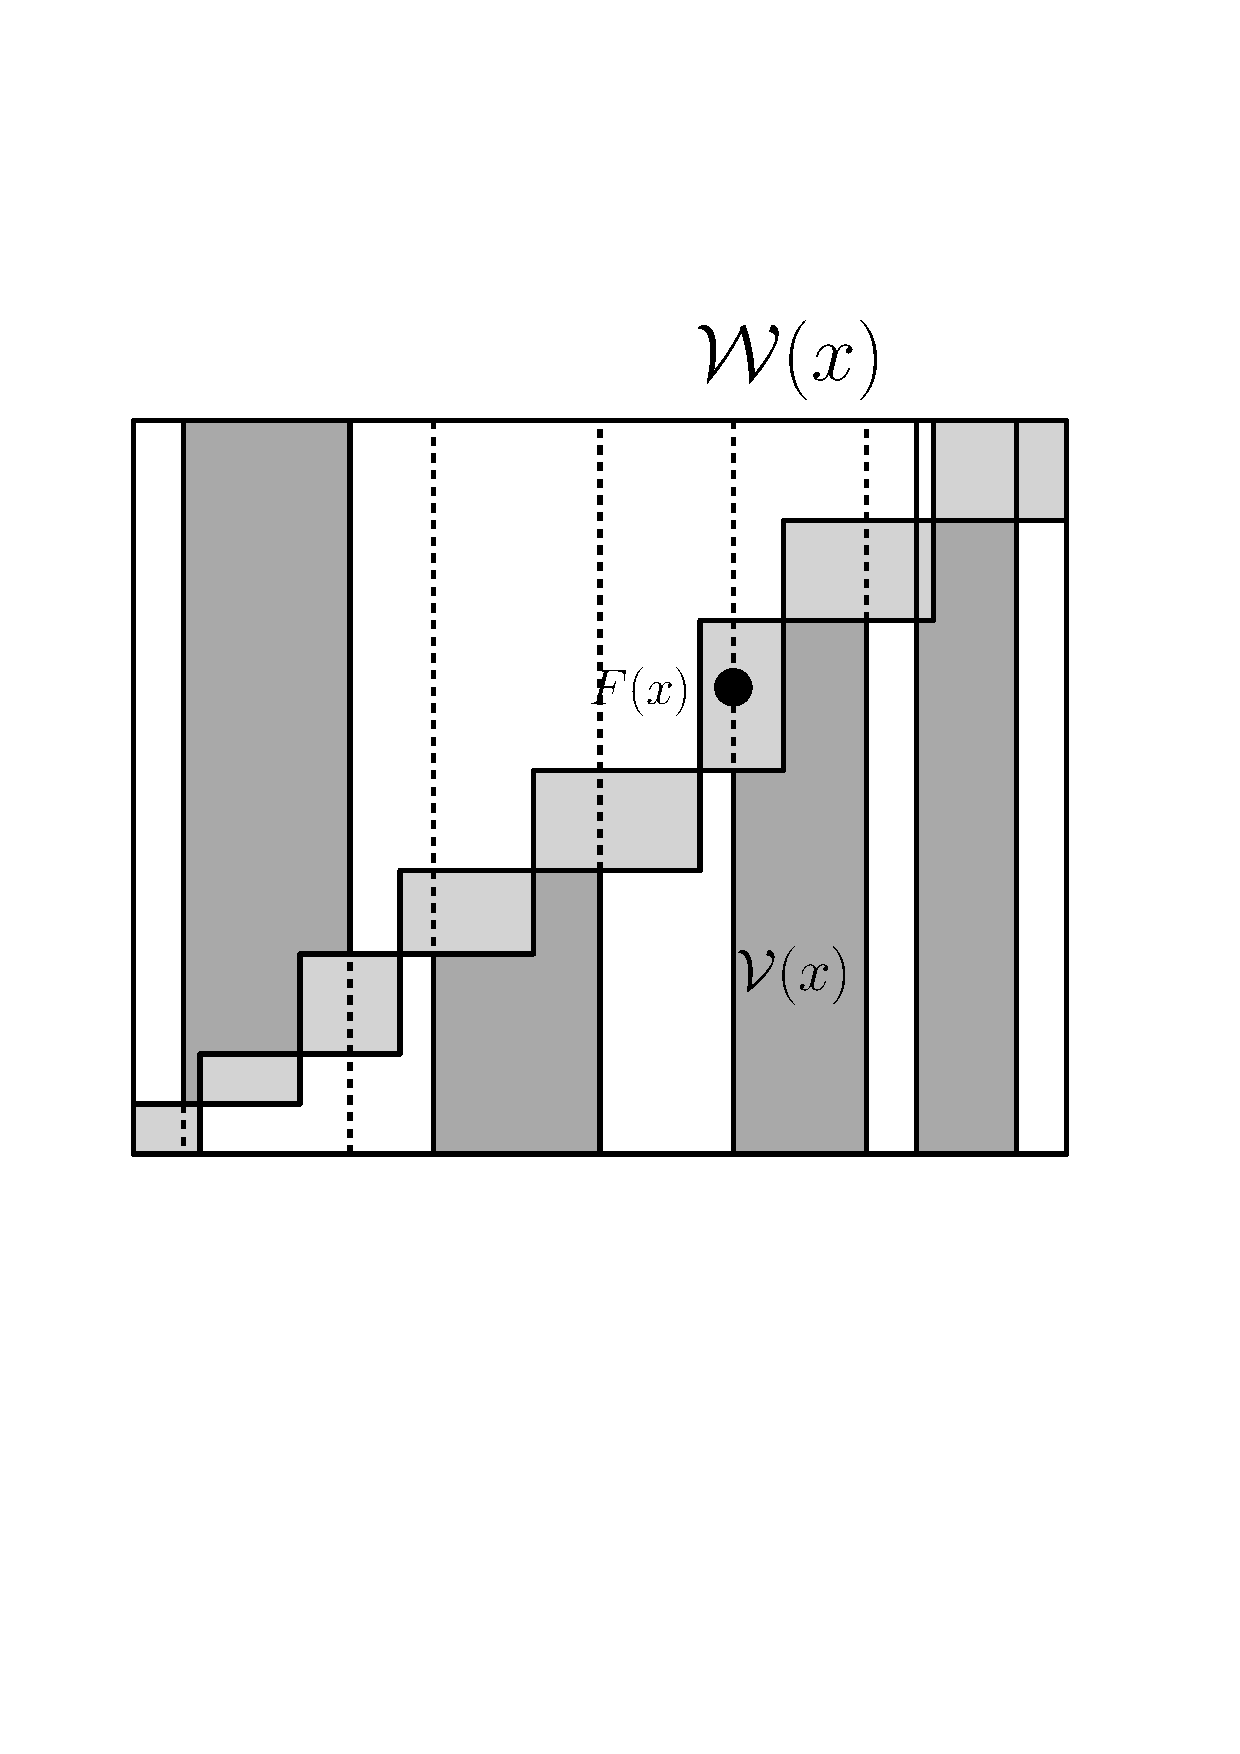
\includegraphics[width=0.2\textwidth]{figures/dichotomy2.pdf}
    \end{center}
    \begin{itemize}
        \item Unsafe points imply a large mass of points MUST lie outside the box chain (in regions $\mathcal{V}(x)$).
        \item If there are few safe points, the total points an increasing sequence can pick up is strictly bounded away from $\chi$.
    \end{itemize}
\end{frame}

\begin{frame}{Building Block 2: Value Nets and Grids}
    \begin{itemize}
        \item To perform the boosting step, we partition a terminal box using a \emph{Grid}.
        \item \textbf{Value Net:} A subset of values $V$ such that any sufficiently "dense" vertical interval contains a point in $V$.
        \begin{center}
            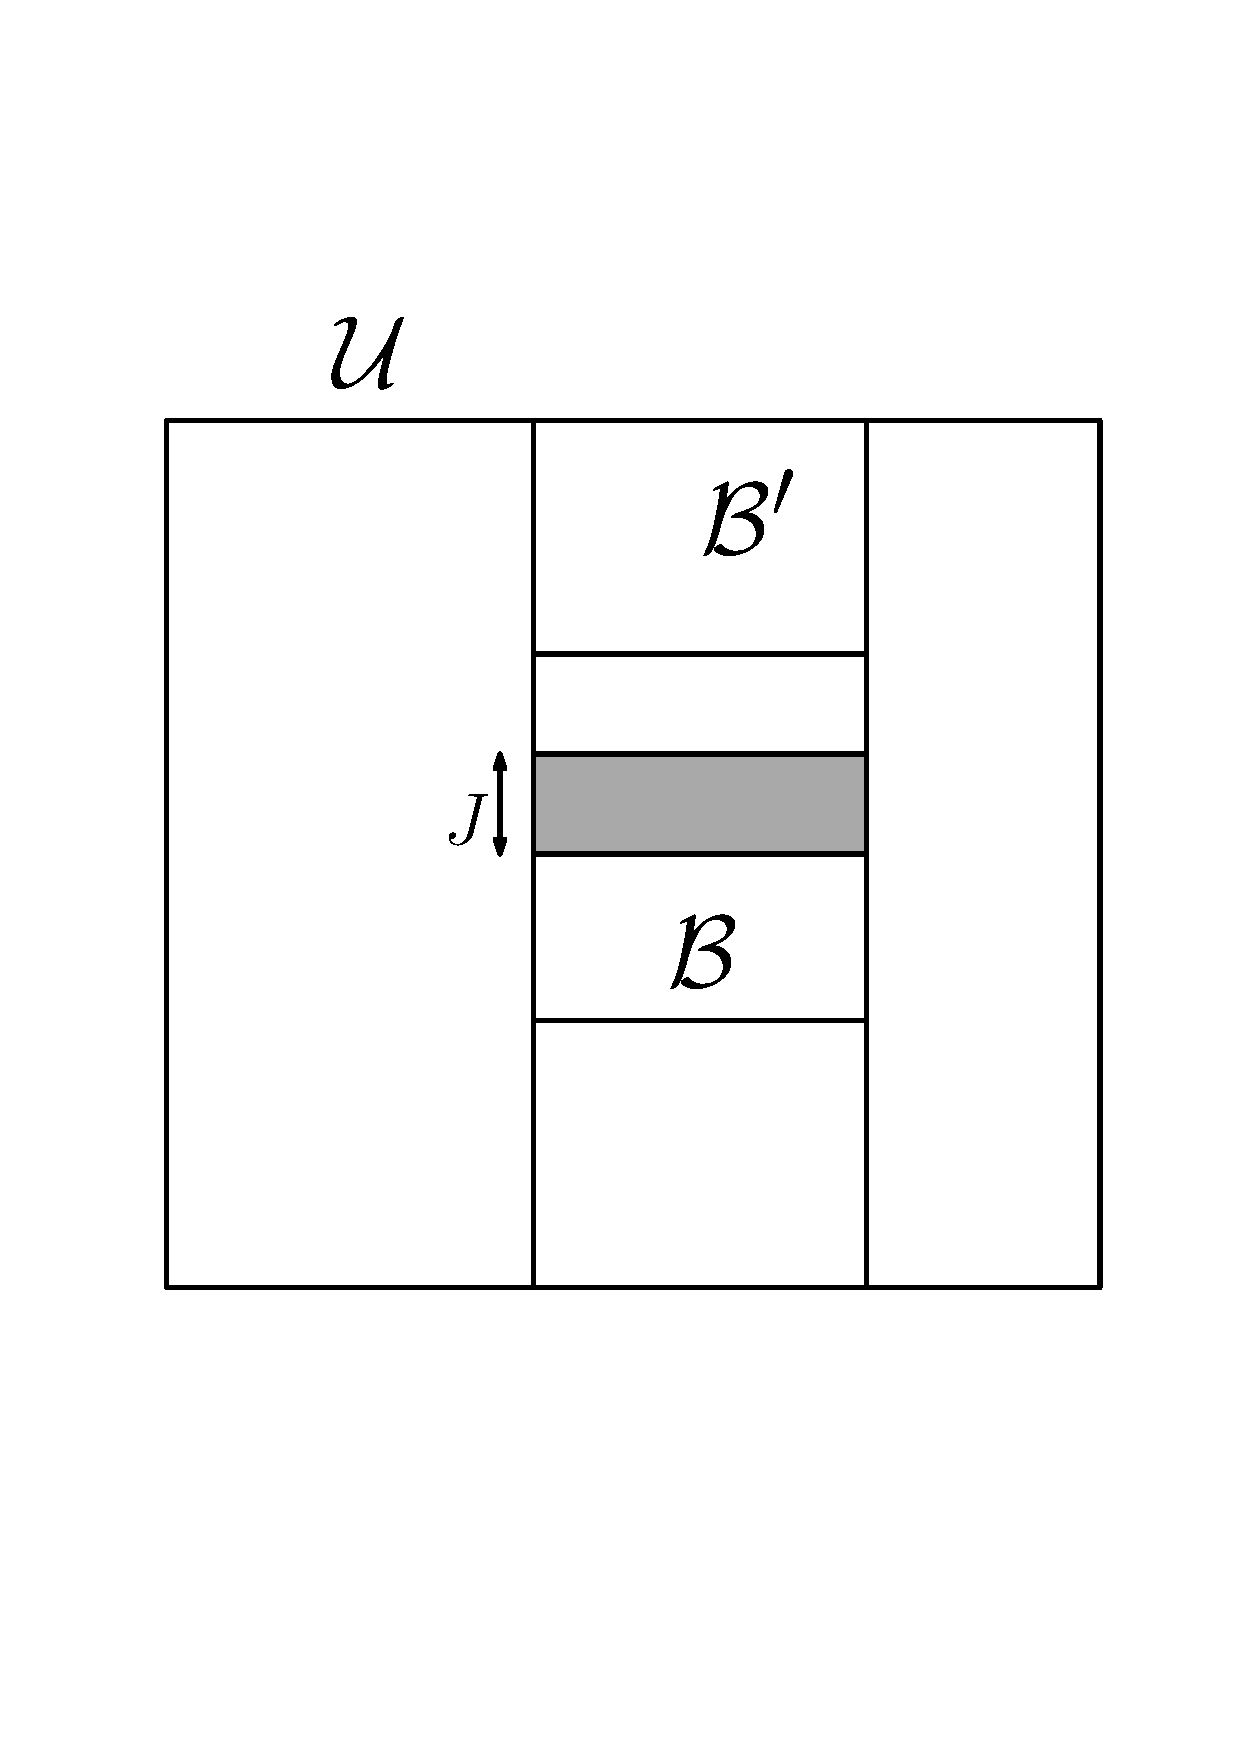
\includegraphics[width=0.2\textwidth]{figures/valuenet.pdf}
        \end{center}
        \item $\buildgrid(\mathcal{B}, \alpha, \xi)$:
        \begin{itemize}
            \item Creates a grid $\Gamma$ with $O(1/\alpha)$ columns and $O(1/\alpha^2)$ rows.
            \item Ensures fine-grained coverage of the points.
        \end{itemize}
    \end{itemize}
\end{frame}

\begin{frame}{The Grid Approximation Lemma}
    \begin{itemize}
        \item We form a Directed Acyclic Graph (DAG) $D(\Gamma)$ over the grid points.
        \item A path in $D(\Gamma)$ corresponds to a sequence of boxes.
        \begin{center}
            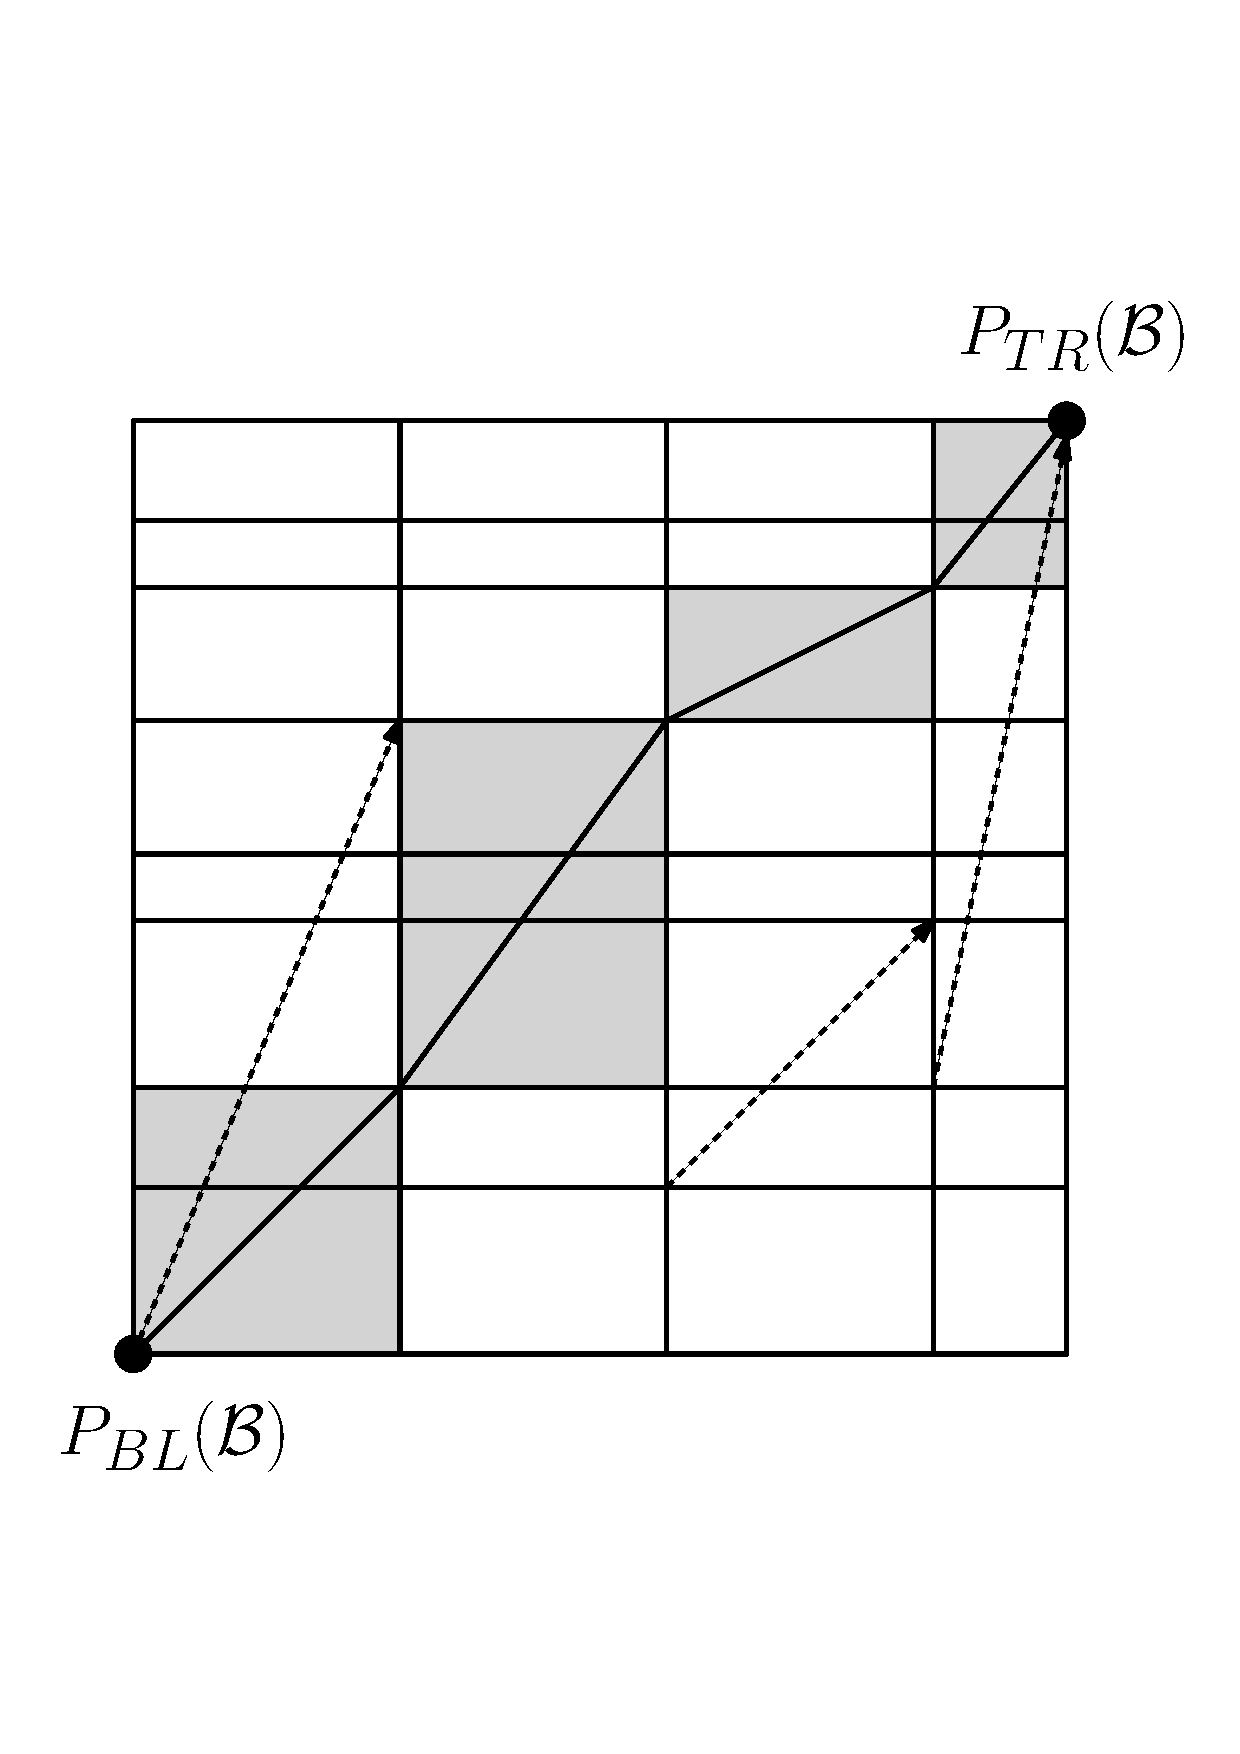
\includegraphics[width=0.2\textwidth]{figures/digraph.pdf}
        \end{center}
    \end{itemize}
    \begin{block}{Lemma 4.9}
        If $\Gamma$ is an $\alpha$-fine grid, then for any increasing sequence $\mathcal{L}$ in $\mathcal{B}$, there is a $D(\Gamma)$-chain $\vec{\mathcal{D}}$ that contains all but $\alpha \cdot \width(\mathcal{B})$ points of $\mathcal{L}$.
    \end{block}
\end{frame}

% =========================================================================
\section{The Basic LIS Approximation Algorithm}
% =========================================================================

\begin{frame}{The Main Procedure: $\approxlis_t(\mathcal{B})$}
    \begin{itemize}
        \item Takes a box $\mathcal{B}$ and a recursion level $t$.
        \item If $\width(\mathcal{B}) = 1$, return $|\mathcal{B} \cap \mathcal{F}|$.
        \item \textbf{Else:}
        \begin{itemize}
            \item Sample $\sigma$ random indices from $X(\mathcal{B})$.
            \item Run $\classify_t(x, \mathcal{B})$ on each sample point $x$.
            \item Let $g$ be the number classified as \emph{good}.
            \item Return $g \cdot \width(\mathcal{B}) / \sigma$.
        \end{itemize}
        \item The entire algorithm hinges on the $\classify$ routine!
    \end{itemize}
\end{frame}

\begin{frame}{The Classify Routine: $\classify_t(x, \mathcal{B})$}
    \begin{itemize}
        \item Goal: Determine if $x$ is "good" or "bad".
        \item If $F(x) \notin \mathcal{B}$, return \emph{bad}.
        \item Base cases ($t=0$ or $\width=1$).
        \item \textbf{Main Step:}
        \begin{enumerate}
            \item Call $\critbox_t(x, \mathcal{B})$ to find a subbox $\mathcal{C}$ containing $x$.
            \item Recursively call $\classify_{t-1}(x, \mathcal{C})$.
            \item Return the result.
        \end{enumerate}
        \item What is the \emph{Critical Box}?
    \end{itemize}
\end{frame}

\begin{frame}{Finding the Critical Box: $\critbox_t(x, \mathcal{B})$}
    \begin{itemize}
        \item Operates in two stages:
        \item \textbf{Stage 1: Terminal Box}
        \begin{itemize}
            \item Run $\terminalbox_t(x, \mathcal{B})$ to simulate the interactive protocol.
            \item Keep finding splitters and shrinking the box around $x$ until $\findsplitter$ fails (or box is tiny).
            \item Returns the \emph{Terminal Box} $\mathcal{T}$.
        \end{itemize}
        \item \textbf{Stage 2: Grid Chain / Boosting}
        \begin{itemize}
            \item Build an $\alpha$-fine grid $\Gamma$ inside $\mathcal{T}$.
            \item For each grid box $\mathcal{D}$, recursively evaluate $\approxlis_{t-1}(\mathcal{D})$ to get a weight.
            \item Find the longest path in $D(\Gamma)$ to get a chain of grid boxes $\vec{\mathcal{C}}(\mathcal{T})$.
            \item Return the unique box $\mathcal{C} \in \vec{\mathcal{C}}(\mathcal{T})$ containing $x$.
        \end{itemize}
    \end{itemize}
\end{frame}

\begin{frame}{Visualizing the Terminal and Critical Chains}
    \begin{center}
        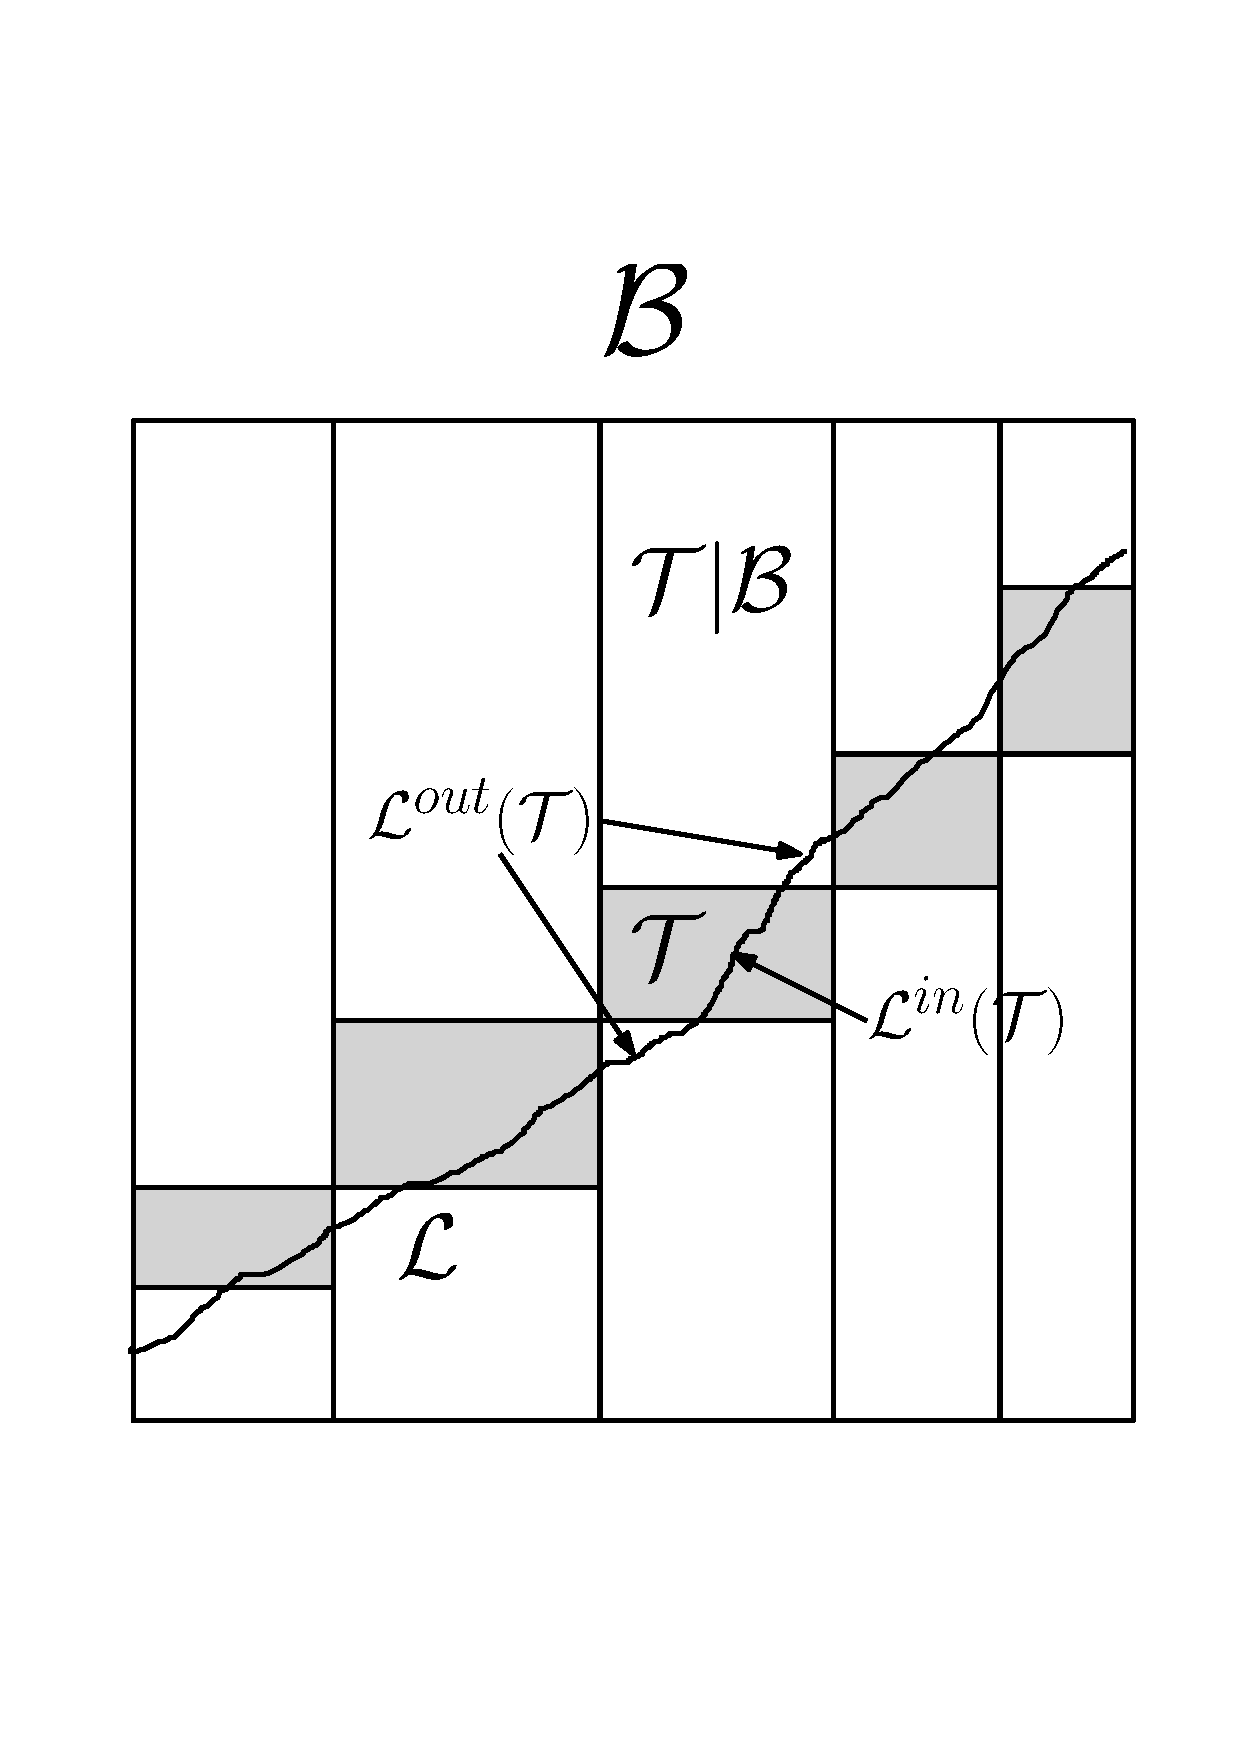
\includegraphics[width=0.2\textwidth]{figures/lis-strip.pdf} \hspace{1cm}
        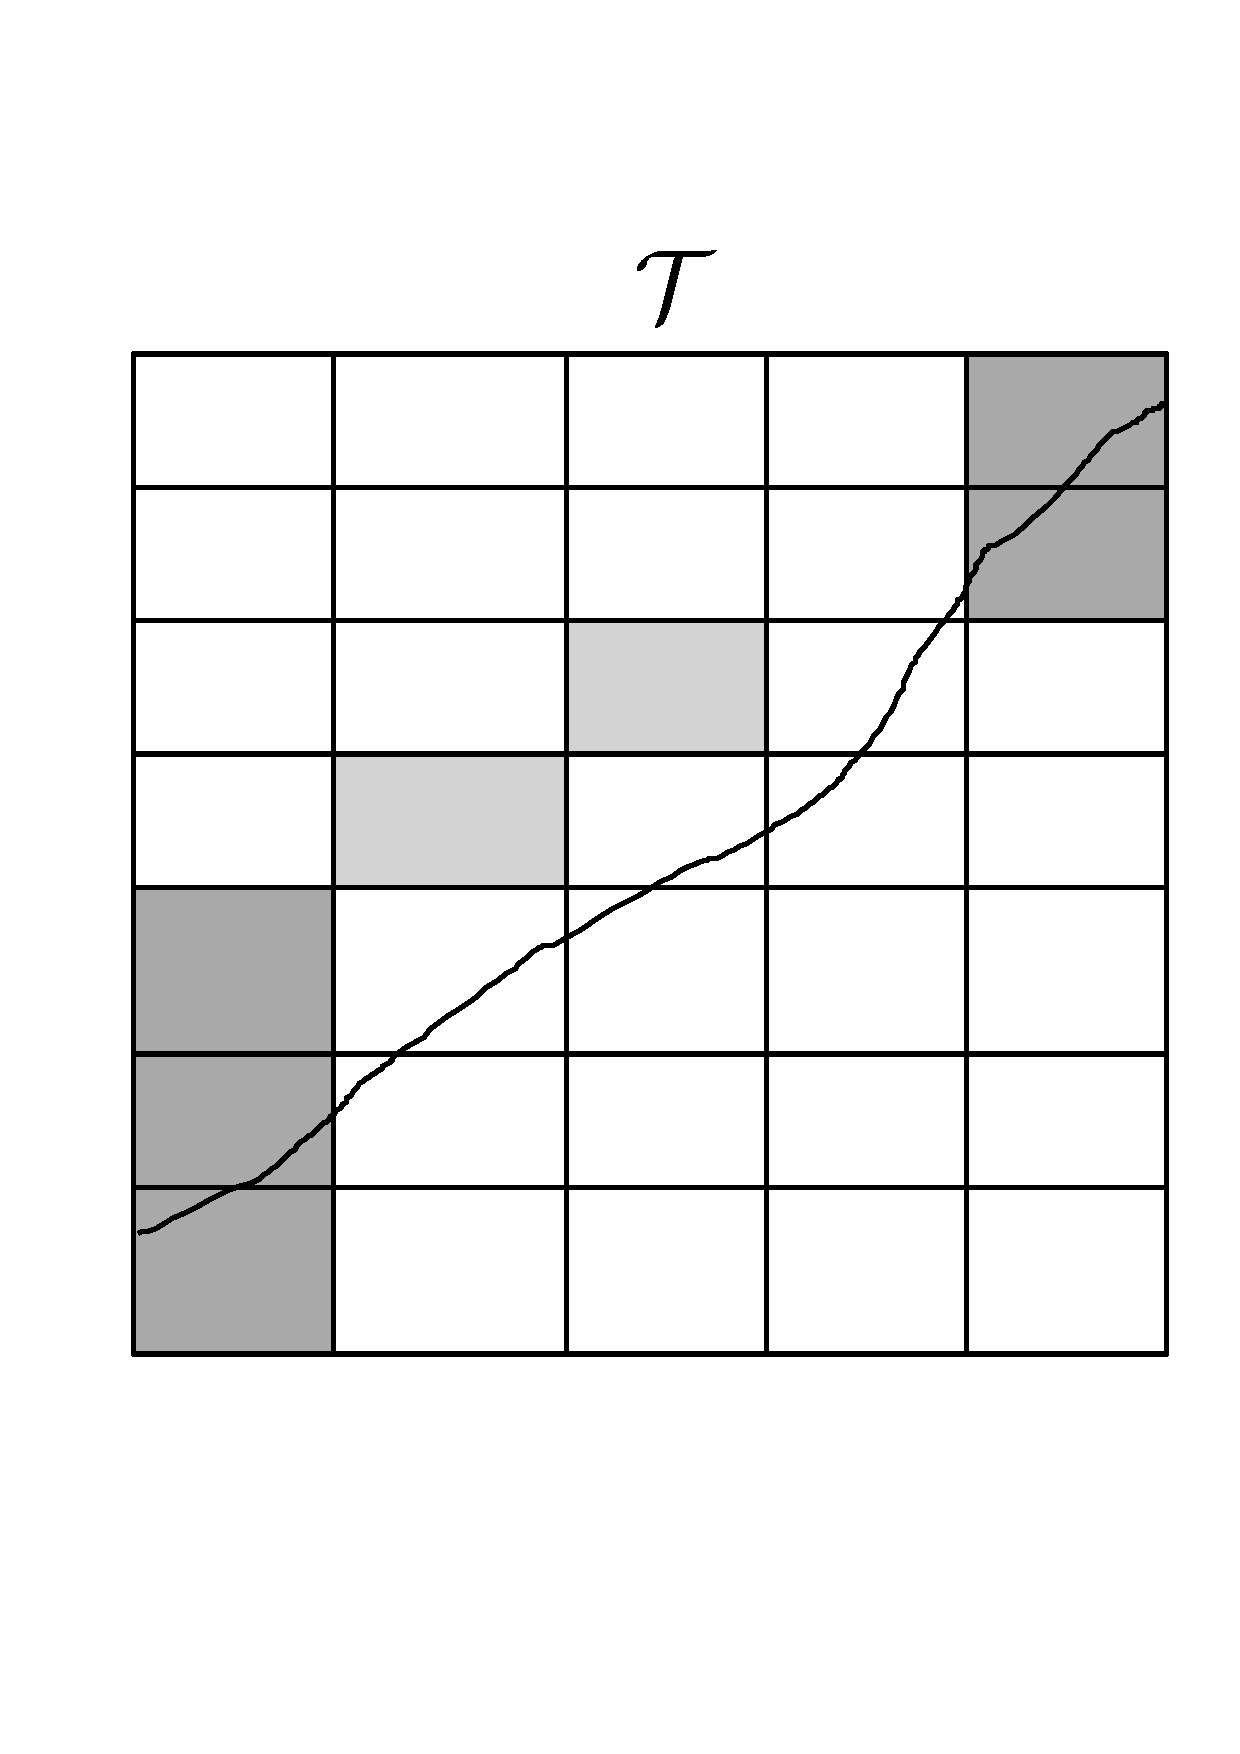
\includegraphics[width=0.2\textwidth]{figures/critical.pdf}
    \end{center}
    \begin{itemize}
        \item Left: $\terminalbox$ partitions the space into nested splits until failure. The leaves are the Terminal Chain.
        \item Right: Inside a terminal box, the Grid Chain solves a DP on grid sub-boxes.
    \end{itemize}
\end{frame}

\begin{frame}{Analysis: The Two Assumptions}
    \begin{itemize}
        \item To analyze the randomized algorithm as deterministic, we fix random bits and assume two properties hold w.h.p.:
        \item \textbf{Assumption 1 (Secondary Randomness):} Every call to $\findsplitter$ and $\buildgrid$ is "reliable" (returns valid splitters/grids if they exist).
        \item \textbf{Assumption 2 (Primary Randomness):} No box-level pair $(\mathcal{B}, t)$ is "tainted".
        \begin{itemize}
            \item Tainted means the sampling in $\approxlis_t$ drastically failed to estimate $|Good_t(\mathcal{B})|$, or errors piled up from children.
        \end{itemize}
        \item Both hold with probability $1 - n^{-\Omega(\log n)}$ using standard Chernoff/Hoeffding bounds.
    \end{itemize}
\end{frame}

\begin{frame}{Error Analysis: Transforming the Goal}
    \begin{itemize}
        \item We want to show: $|\lis(\mathcal{B}) - \approxlis_t(\mathcal{B})| \leq \tau_t \loss(\mathcal{B}) + \delta_t \width(\mathcal{B})$.
        \item We define a discrepancy metric for a terminal box $\mathcal{T}$:
        $$\Delta_t(\mathcal{T}) = (1+\tau_t)|\mathcal{L}(\mathcal{T})| - |Good_t(\mathcal{B}) \cap \mathcal{T}| - \tau_t \beta(\mathcal{T})$$
        \item We bound the error by splitting it into \emph{Primary Error} (involving $\tau_t, \loss$) and \emph{Secondary Error} (involving $\delta_t$, sampling bounds).
    \end{itemize}
\end{frame}

\begin{frame}{Secondary Error Terms}
    \begin{itemize}
        \item We identify 5 sources of error:
        \begin{enumerate}
            \item $\epsilon_1$: Sampling error in estimating $|Good_t|$.
            \item $\epsilon_2$: Cumulative error from $\approxlis_{t-1}$ calls.
            \item $\epsilon_3$: Points of the true LIS lost because they fall outside the chosen grid chain.
            \item $\epsilon_4$: Points of the true LIS lost because they violate the chosen splitters.
            \item $\epsilon_5$: Loss accounted for by the Dichotomy Lemma inside terminal boxes.
        \end{enumerate}
        \item We prove each term is bounded by $O(\delta \width(\mathcal{B}))$.
    \end{itemize}
\end{frame}

\begin{frame}{Recurrences for $\tau_t$ and $\mu_t$}
    \begin{itemize}
        \item Setting up the algebraic inequalities requires balancing the primary error terms.
        \item To force the primary error to contract at each recursive level, we must set:
        $$\mu_t = \frac{\tau_{t-1}}{2(1+\tau_{t-1})}$$
        \item This yields the recurrence:
        $$\tau_t \geq \left( \frac{2\tau_{t-1}+2}{\tau_{t-1}+2} \right)^2 - 1$$
        \item A solution to this is $\tau_t = 4/t$ and $\mu_t = 2/(t+3)$.
        \item Note: As $t \to \infty$, $\tau_t \to 0$, achieving arbitrary multiplicative precision on the loss!
    \end{itemize}
\end{frame}

% =========================================================================
\section{The Improved Algorithm}
% =========================================================================

\begin{frame}{Bottleneck of the Basic Algorithm}
    \begin{itemize}
        \item Running time of basic algorithm is $O(\log n)^{O(1/\tau)}$.
        \item Why? At each recursive level, we create a grid of size $\text{poly}(\log n)$ and make recursive calls.
        \item The depth is $t_{\max} = O(1/\tau)$.
        \item $(\log n)$ to the power of $(1/\tau)$ is strictly sublinear, but not purely polylogarithmic in terms of exponent independence.
        \item We want $(1/\epsilon)^{O(1/\tau)} \log^c n$. The exponent of $\log n$ should be a constant!
    \end{itemize}
\end{frame}

\begin{frame}{The Core Innovation: Phases in TerminalBox}
    \begin{itemize}
        \item In the basic algorithm, if $\findsplitter$ fails, we declare a terminal box immediately.
        \item In the improved algorithm, we introduce \textbf{Phases}.
        \item If $\findsplitter$ fails, we don't stop. We increment a phase counter $j$, and \emph{relax} the splitter constraints:
        \begin{itemize}
            \item Increase the violation allowance $\gamma \to \gamma_j$.
            \item Tighten the balance requirement $\rho \to \rho_j$.
            \item Increase the width threshold $\theta$.
        \end{itemize}
        \item We only terminate when the box width drops below the threshold $\theta$.
    \end{itemize}
\end{frame}

\begin{frame}{The Improved TerminalBox Algorithm}
    \begin{algorithmic}[1]
        \State $j \gets 0$, $\theta \gets \omega$, $\gamma \gets \gamma_0$, $\rho \gets \rho_0$
        \While{$\width(\mathcal{T}) > \theta$}
            \State Run $\findsplitter(\mathcal{T}, \dots, \gamma, \rho)$
            \If{splitter found}
                \State Split $\mathcal{T}$ based on $x$'s position.
            \Else
                \State \textbf{New Phase!}
                \State $\theta \gets \max(\theta, \gamma \width(\mathcal{T}) / \alpha)$
                \State $j \gets j + 1$
                \State $\gamma \gets \gamma_j$, $\rho \gets \rho_j$
            \EndIf
        \EndWhile
    \end{algorithmic}
\end{frame}

\begin{frame}{Why do Phases Help?}
    \begin{itemize}
        \item In the basic algorithm, the grid precision $\alpha$ was tied directly to $\gamma$, which had to be $\sim 1/\log n$.
        \item By progressively relaxing $\gamma_j$, we can decouple the grid precision $\alpha$ from $\log n$.
        \item We can set the grid precision $\alpha$ to be polynomial in an \emph{error controller} $\Psi$, completely independent of $n$.
        \item This ensures the branching factor in the recursion relies only on $\Psi$, not on $\log n$.
        \item Result: Exponent of $\log n$ drops to a constant $c$.
    \end{itemize}
\end{frame}

\begin{frame}{Revisiting Tainted Boxes}
    \begin{itemize}
        \item Since we lowered the sample size to rely on $\Psi$ instead of $\log n$, we can no longer use a simple union bound over all possible boxes.
        \item A single call might fail with non-negligible probability.
        \item We handle this by proving that errors do not cascade catastrophically.
        \item \textbf{Lemma 9.7:} The probability that any box-level pair is recursively "tainted" is bounded by a carefully controlled polynomial in $\alpha$.
        \item The expected mass of blue (tainted) sub-grids remains strictly bounded, preserving the global LIS estimate.
    \end{itemize}
\end{frame}

\begin{frame}{Final Time Complexity}
    \begin{itemize}
        \item Maximum recursion depth: $t_{\max} = \lceil 4/\tau \rceil$.
        \item Error controller: $\Psi = \max(C, t_{\max}/\delta)$.
        \item Branching factor per node: $\text{poly}(\Psi)$.
        \item Running time: $O(\Psi^{O(t_{\max})} \log^c n)$.
        \item Substituting parameters: $(1/\delta\tau)^{O(1/\tau)} \log^c n$.
        \item The dependence on the array size $n$ is purely $\log^c n$.
    \end{itemize}
\end{frame}

% =========================================================================
\section{Conclusion}
% =========================================================================

\begin{frame}{Summary of the Paper}
    \begin{itemize}
        \item First polylogarithmic time algorithm for an \textbf{additive approximation} of LIS.
        \item Improved distance to monotonicity estimation from $(2+o(1))$ to $(1+\tau)$.
        \item \textbf{Key Techniques:}
        \begin{itemize}
            \item Simulating Interactive Protocols without an Oracle.
            \item Dichotomy between conservative splitters and approximation boosting.
            \item Recursive dynamic programming on localized grids.
            \item Dynamic phase relaxation to decouple structural parameters from $n$.
        \end{itemize}
        \item A powerful framework for approximating DP problems in sublinear time!
    \end{itemize}
\end{frame}

\begin{frame}{Questions?}
    \begin{center}
        \Huge Thank You!
    \end{center}
    \vspace{1cm}
    \begin{center}
        Estimating the Longest Increasing Sequence in Polylogarithmic Time \\
        M. Saks and C. Seshadhri
    \end{center}
\end{frame}

\end{document}
